% Options for packages loaded elsewhere
\PassOptionsToPackage{unicode}{hyperref}
\PassOptionsToPackage{hyphens}{url}
%
\documentclass[
]{article}
\usepackage{lmodern}
\usepackage{amssymb,amsmath}
\usepackage{ifxetex,ifluatex}
\ifnum 0\ifxetex 1\fi\ifluatex 1\fi=0 % if pdftex
  \usepackage[T1]{fontenc}
  \usepackage[utf8]{inputenc}
  \usepackage{textcomp} % provide euro and other symbols
\else % if luatex or xetex
  \usepackage{unicode-math}
  \defaultfontfeatures{Scale=MatchLowercase}
  \defaultfontfeatures[\rmfamily]{Ligatures=TeX,Scale=1}
\fi
% Use upquote if available, for straight quotes in verbatim environments
\IfFileExists{upquote.sty}{\usepackage{upquote}}{}
\IfFileExists{microtype.sty}{% use microtype if available
  \usepackage[]{microtype}
  \UseMicrotypeSet[protrusion]{basicmath} % disable protrusion for tt fonts
}{}
\makeatletter
\@ifundefined{KOMAClassName}{% if non-KOMA class
  \IfFileExists{parskip.sty}{%
    \usepackage{parskip}
  }{% else
    \setlength{\parindent}{0pt}
    \setlength{\parskip}{6pt plus 2pt minus 1pt}}
}{% if KOMA class
  \KOMAoptions{parskip=half}}
\makeatother
\usepackage{xcolor}
\IfFileExists{xurl.sty}{\usepackage{xurl}}{} % add URL line breaks if available
\IfFileExists{bookmark.sty}{\usepackage{bookmark}}{\usepackage{hyperref}}
\hypersetup{
  pdftitle={Supplementary Information},
  hidelinks,
  pdfcreator={LaTeX via pandoc}}
\urlstyle{same} % disable monospaced font for URLs
\usepackage[margin=1in]{geometry}
\usepackage{graphicx,grffile}
\makeatletter
\def\maxwidth{\ifdim\Gin@nat@width>\linewidth\linewidth\else\Gin@nat@width\fi}
\def\maxheight{\ifdim\Gin@nat@height>\textheight\textheight\else\Gin@nat@height\fi}
\makeatother
% Scale images if necessary, so that they will not overflow the page
% margins by default, and it is still possible to overwrite the defaults
% using explicit options in \includegraphics[width, height, ...]{}
\setkeys{Gin}{width=\maxwidth,height=\maxheight,keepaspectratio}
% Set default figure placement to htbp
\makeatletter
\def\fps@figure{htbp}
\makeatother
\setlength{\emergencystretch}{3em} % prevent overfull lines
\providecommand{\tightlist}{%
  \setlength{\itemsep}{0pt}\setlength{\parskip}{0pt}}
\setcounter{secnumdepth}{-\maxdimen} % remove section numbering
\usepackage{float} \usepackage{caption} \captionsetup[table]{font=footnotesize} \captionsetup[figure]{font=footnotesize} \captionsetup[figure]{labelformat=empty} \captionsetup[table]{labelformat=empty} \usepackage{pdflscape} \newcommand{\blandscape}{\begin{landscape}} \newcommand{\elandscape}{\end{landscape}}
\usepackage{booktabs}
\usepackage{longtable}
\usepackage{array}
\usepackage{multirow}
\usepackage{wrapfig}
\usepackage{float}
\usepackage{colortbl}
\usepackage{pdflscape}
\usepackage{tabu}
\usepackage{threeparttable}
\usepackage{threeparttablex}
\usepackage[normalem]{ulem}
\usepackage{makecell}
\usepackage{xcolor}

\title{Supplementary Information}
\author{}
\date{\vspace{-2.5em}}

\begin{document}
\maketitle

{
\setcounter{tocdepth}{3}
\tableofcontents
}
\newpage

\hypertarget{appendix-s1.-methods-for-reconstruction-of-dbh}{%
\subsection{\texorpdfstring{Appendix S1. Methods for reconstruction of
\(DBH\)}{Appendix S1. Methods for reconstruction of DBH}}\label{appendix-s1.-methods-for-reconstruction-of-dbh}}

For each core, \(DBH\) can be reconstructed outside-in (based on recent
\(DBH\), subtracting growth recorded in tree rings) or inside-out
(summing \(\Delta r\) from the inside out). We generally gave precedence
to the outside-in approach. Specifically, when \(DBH\) was taken at the
time of coring,\\
At some of our sites where DBH was not taken at the time of coring
(\emph{SCBI},), DBH measurements taken before or slightly after the time
of coring could be used. (see
\href{https://github.com/EcoClimLab/ForestGEO_dendro/issues/19}{issue
\#19 in ForestGEO\_dendro}) If before, \ldots{} If after\ldots{} For all
outside-in reconstructions, if a negative \(DBH\) was predicted\ldots{}

When there were more than one cores for a tree, the \(DBH\)
reconstructions from each core were averaged to produce a single
estimate of the tree's \(DBH\) through time. When the start or end dates
of the records from the cores differed, we extrapolated growth of the
shorter core to match the years covered by the longer core.
Specifically, to fill in years at the more recent end, we assumed that
the average growth rate of the ten years prior to the missing records
applied to the missing years. To fill in years at the beginning of the
tree's lifespan, we likewise assumed that the ten years adjacent to the
missing record applied to the missing years; however, if this yielded a
negative \(DBH\) estimate for the earliest year in the reconstruction,
we divided the existing minimum \(DBH\) by number of years missing and
applied that value to each year. We note that these reconstructed growth
records were used only for the reconstruction of \(DBH\) and were not
included as response variables in any of our analyses.

In either case we need bark thickness--ideally allometries describing
the relationship between DBH and bark thickness (Table S4). This is
especially critical for thick-barked species When bark thickness data
were available, we generated allometries \ldots{} lognormal model with
intercept forced to zero: lm(bark\_depth.mm \textasciitilde{} -1 +
log(dbh\_no\_bark.cm+1):bark\_species, data = bark)
(\href{https://github.com/EcoClimLab/ForestGEO_dendro/issues/8}{issue
\#8 in ForestGEO\_dendro})

\newpage

\hypertarget{appendix-s2.-methods-for-comparing-climwin-results-with-traditional-methods}{%
\subsection{Appendix S2. Methods for comparing climwin results with
traditional
methods}\label{appendix-s2.-methods-for-comparing-climwin-results-with-traditional-methods}}

(**\href{https://github.com/EcoClimLab/ForestGEO-climate-sensitivity/issues/35}{ISSUE
\#35 in ForestGEO-climate-sensitivity}

\newpage

\hypertarget{appendix-s3.-dealing-with-rapidly-changing-climate-and-tree-growth}{%
\subsection{Appendix S3. Dealing with rapidly changing climate and tree
growth}\label{appendix-s3.-dealing-with-rapidly-changing-climate-and-tree-growth}}

\href{https://github.com/EcoClimLab/ForestGEO-climate-sensitivity/issues/25}{ISSUE
\#25 in ForestGEO-climate-sensitivity}

Our analysis included two sites where climate change has had pronounced
effects on tree growth: Scotty Creek, NW Territories, Canada (SC) and
Little Tesuque, New Mexico, USA (LT). At SC, {[}temperatures have
increased by X \(^\circ\) over X years{]}\ldots, resulting in negative
growth trends in basal area index (\(BAI\)) starting around 1950 and
significant growth declines since 1970 in 56\% of trees
{[}@sniderhan\_growth\_2016{]}.

\newpage

\hypertarget{table-s1.-site-details}{%
\subsection{Table S1. Site Details}\label{table-s1.-site-details}}

\begin{table}[!h]
\centering
\resizebox{\linewidth}{!}{
\begin{tabular}{l>{\raggedright\arraybackslash}p{3cm}rr>{\raggedright\arraybackslash}p{2cm}>{\raggedright\arraybackslash}p{1.5cm}llll}
\toprule
site code & site name & latitude & longitude & cores within ForestGEO plot? & canopy positions & tree statuses & date range & dormant season & months in climwin\\
\midrule
BCI & Barro Colorado Island & 9.15430 & -79.8461 & no & canopy & live, dead & 1931-2014 & Nov-Apr & pOct-cDec\\
HKK & Huai Kha Khaeng & 15.63240 & 99.2170 & no & all & live & 1903-2011 &  & pOct-cDec\\
LT & Little Tesuque & 35.73838 & -105.8382 & n.a. & all & live & 1903-2018 &  & pMay-cAug\\
CB & Utah Forest Dynamics Plot & 37.66150 & -112.8525 &  &  &  & 1903-2007 &  & pMay-cAug\\
SCBI & Smithsonian Conservation Biology Institute & 38.89350 & -78.1454 & yes & all & live, dead & 1903-2017 & Oct-Apr & pMay-cAug\\
\addlinespace
LDW & Lilly Dickey Woods & 39.23590 & -86.2181 &  & canopy & live, dead & 1903-2019 &  & pMay-cAug\\
HF & Harvard Forest & 42.53880 & -72.1755 & yes & all & live, dead & 1903-2014 &  & pMay-cAug\\
NB & Niobrara/Hansley & 42.78000 & -100.0210 &  &  &  &  &  & pMay-cAug\\
ZOF & Zofin Forest Dynamics Plot & 48.66380 & 14.7073 & some & all &  & 1903-2013 &  & pMay-cAug\\
SC & Scotty Creek & 61.30000 & -121.3000 & no & all & live, dead & 1903-2013 &  & pMay-cAug\\
\bottomrule
\end{tabular}}
\end{table}

\newpage

\hypertarget{table-s2.-species-analyzed-their-characteristics-and-bark-allometries-applied}{%
\subsection{Table S2. Species analyzed, their characteristics, and bark
allometries
applied}\label{table-s2.-species-analyzed-their-characteristics-and-bark-allometries-applied}}

(**\href{https://github.com/EcoClimLab/ForestGEO-climate-sensitivity/issues/72}{ISSUE
\#72 in ForestGEO-climate-sensitivity}

\begin{table}[!h]
\centering
\resizebox{\linewidth}{!}{
\begin{tabular}{llllllll}
\toprule
species code & family & latin name & site(s) sampled & leaf type & leaf phenology & light requirements & bark allometry*\\
\midrule
$species_code in sitespecies.csv$ & family in sitespecies.csv & $latin_name$ in sitespecies.csv & site codes & $leaf_type$ in sitespecies.csv & $leaf_phenology$ in sitespecies.csv & $light_requirements$ in sitespecies.csv & "$bark_species$ in $bark_site$"\\
\bottomrule
\end{tabular}}
\end{table}

*Bark allometry field indicates the species and site sampled to
construct the bark allometry. When neither raw data nor an allometric
equation for the study species was available, we selected the most
appropriate equation that could be located for similar species.
Equations are given in Table S4.

\newpage

\hypertarget{table-s3.-sampling-details-for-species-by-site}{%
\subsection{Table S3. Sampling details for species by
site}\label{table-s3.-sampling-details-for-species-by-site}}

(**\href{https://github.com/EcoClimLab/ForestGEO-climate-sensitivity/issues/73}{ISSUE
\#73 in ForestGEO-climate-sensitivity}

\newpage

\hypertarget{table-s4.-allometric-equations-for-bark-thickness}{%
\subsection{Table S4. Allometric equations for bark
thickness}\label{table-s4.-allometric-equations-for-bark-thickness}}

(**\href{https://github.com/EcoClimLab/ForestGEO-climate-sensitivity/issues/71}{ISSUE
\#71 in ForestGEO-climate-sensitivity}

\begin{table}[!h]
\centering
\resizebox{\linewidth}{!}{
\begin{tabular}{llrlll}
\toprule
species & equation & n & DBH_range_cm & site & source\\
\midrule
Picea mariana & bark_mm ~ 3.72623722229494 x log(dbh_cm + 1) & 12 & 6.9-7.9 & Scotty Creek & Anastasia Sniderhan & Jennifer Baltzer, unpublished data\\
Acer rubrum & bark_mm ~ 0.619247869059281 x log(dbh_cm + 1) & 10 & 8.2-39.6 & SCBI & Anderson-Teixeira et al. 2015\\
Carya cordiformis & bark_mm ~ 0.792634265459979 x log(dbh_cm + 1) & 9 & 5.9-68.2 & SCBI & Anderson-Teixeira et al. 2015\\
Carya ovata & bark_mm ~ 1.03526537862387 x log(dbh_cm + 1) & 8 & 19.1-78 & SCBI & Anderson-Teixeira et al. 2015\\
Carya ovalis & bark_mm ~ 1.53091027316465 x log(dbh_cm + 1) & 8 & 6.4-63.1 & SCBI & Anderson-Teixeira et al. 2015\\
\addlinespace
Carya tomentosa & bark_mm ~ 1.10516754737747 x log(dbh_cm + 1) & 8 & 5-57.3 & SCBI & Anderson-Teixeira et al. 2015\\
Fraxinus americana & bark_mm ~ 2.22258328551736 x log(dbh_cm + 1) & 9 & 6.1-94.2 & SCBI & Anderson-Teixeira et al. 2015\\
Juglans nigra & bark_mm ~ 2.10650701999149 x log(dbh_cm + 1) & 9 & 13.6-85.4 & SCBI & Anderson-Teixeira et al. 2015\\
Liriodendron tulipifera & bark_mm ~ 1.63704813876961 x log(dbh_cm + 1) & 9 & 27.5-136.5 & SCBI & Anderson-Teixeira et al. 2015\\
Quercus alba & bark_mm ~ 1.8284678911941 x log(dbh_cm + 1) & 10 & 9.3-101.8 & SCBI & Anderson-Teixeira et al. 2015\\
\addlinespace
Quercus montana & bark_mm ~ 2.08318335755429 x log(dbh_cm + 1) & 8 & 5.8-99.1 & SCBI & Anderson-Teixeira et al. 2015\\
Quercus rubra & bark_mm ~ 0.980268506421506 x log(dbh_cm + 1) & 10 & 24.1-143.2 & SCBI & Anderson-Teixeira et al. 2015\\
Quercus velutina & bark_mm ~ 1.393527450698 x log(dbh_cm + 1) & 8 & 16.2-110.7 & SCBI & Anderson-Teixeira et al. 2015\\
Pinus strobus & bark_mm ~ 1.56758602437827 x log(dbh_cm + 1) & 1 & 28.4-28.4 & Illinois & Miles & Smith (2009)\\
Trichilia tuberculata & bark_mm ~ 1.36652255956719 x log(dbh_cm + 1) & 7 & 21-30.2 & Panama & Pete Kerby-Miller & Helene Muller-Landau, unpublished data\\
\addlinespace
Jacaranada copaia & bark_mm ~ 2.99321697140489 x log(dbh_cm + 1) & 5 & 45.6-75 & Panama & Raquel Alfaro-Sanchez, unpublished data\\
Tetragastris panamensis & bark_mm ~ 1.67185680741063 x log(dbh_cm + 1) & 4 & 22.7-48.8 & Panama & Raquel Alfaro-Sanchez, unpublished data\\
Trichilia tuberculata & bark_mm ~ 1.36652255956719 x log(dbh_cm + 1) & 5 & 28.3-40.5 & Panama & Raquel Alfaro-Sanchez, unpublished data\\
Pseudotsuga menziesii & bark_mm ~  (0.785*sqrt(dbh_cm))^2 & 30 & ~10-200 & California (3 montane sites) & Zeibig-Kichas, 2016, table 3\\
Pinus ponderosa & bark_mm ~  (1.298*sqrt(dbh_cm)^0.802)^2 & 81 & ~5-160 & California (4 montane sites) & Zeibig-Kichas, 2016, table 3\\
\addlinespace
Pinus flexilis & bark_mm ~  (1.299*sqrt(dbh_cm)^0.609)^2 & 29 & ~10-130 & California (3 montane sites) & Zeibig-Kichas, 2016, table 3\\
\bottomrule
\end{tabular}}
\end{table}

\newpage

\hypertarget{table-s5.-frequency-of-dbh-climate-interactions-across-all-sites-and-growth-metrics}{%
\subsection{\texorpdfstring{Table S5. Frequency of \(DBH\)-climate
interactions across all sites and growth
metrics}{Table S5. Frequency of DBH-climate interactions across all sites and growth metrics}}\label{table-s5.-frequency-of-dbh-climate-interactions-across-all-sites-and-growth-metrics}}

\newpage

\hypertarget{figure-s1.-comparison-of-our-approach-with-traditional-methods-of-identifying-climate-signals}{%
\subsection{Figure S1. Comparison of our approach with traditional
methods of identifying climate
signals}\label{figure-s1.-comparison-of-our-approach-with-traditional-methods-of-identifying-climate-signals}}

\begin{figure}
\centering
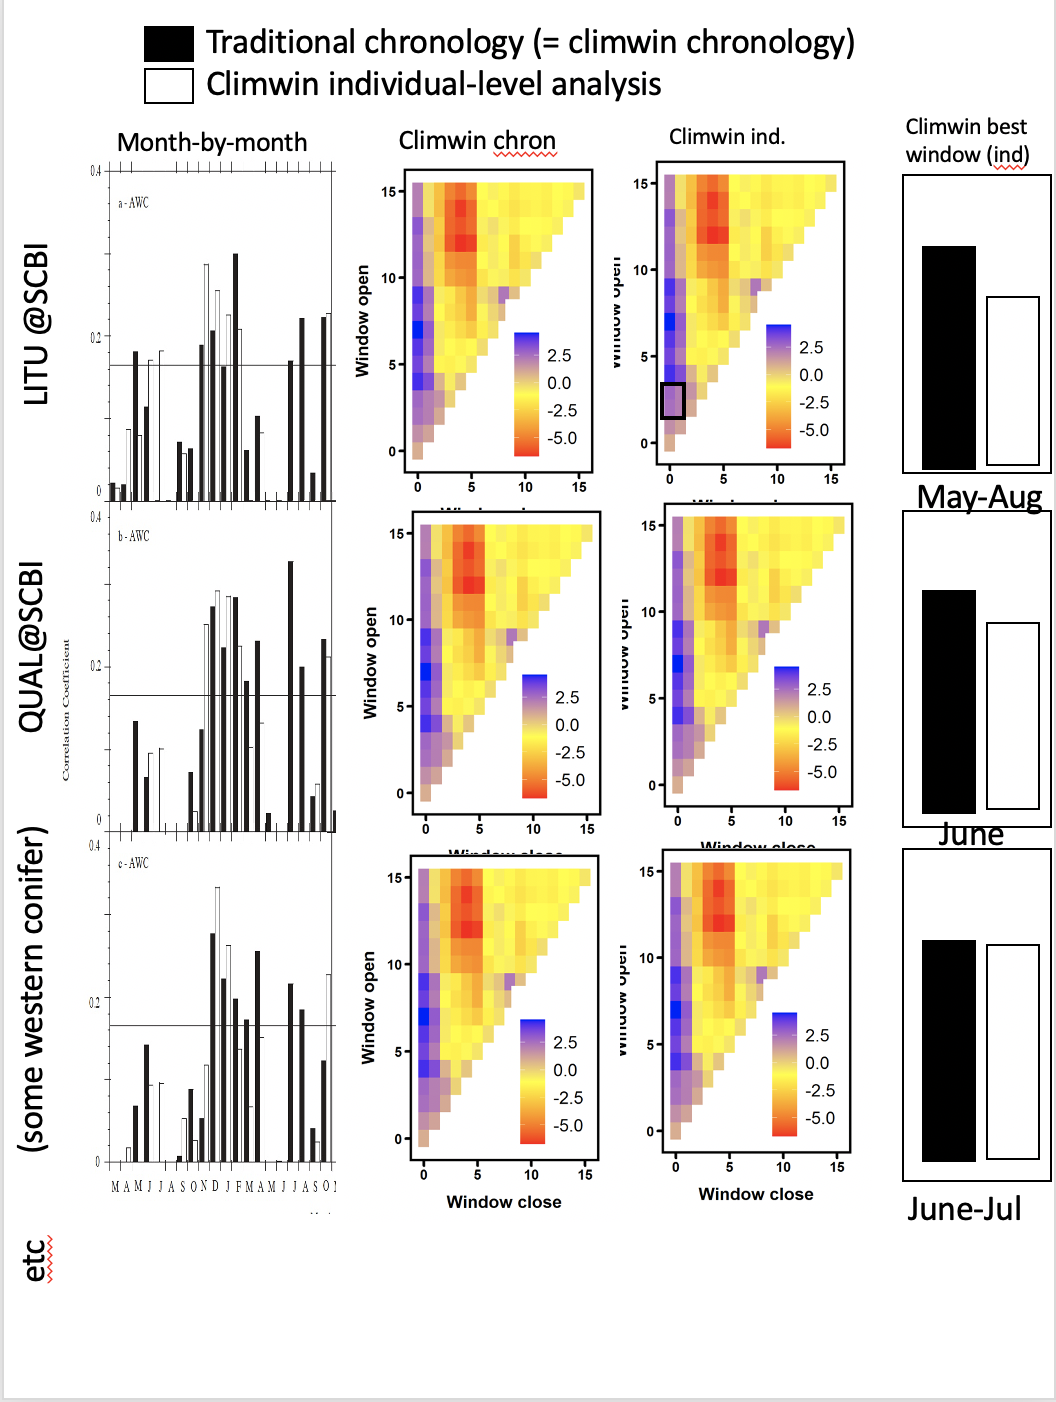
\includegraphics[width=0.7\textwidth,height=\textheight]{tables_figures/mock_comparison_traditional_method.png}
\caption{\textbf{Figure S1 \textbar{} (Comparison of traditional
approaches with ours).} (THIS FIGURE IS JUST A MOCK-UP TO SHOW VALENTINE
WHAT I HAVE IN MIND.)}
\end{figure}

\newpage

\hypertarget{figure-s2.-comparison-of-climwin-output-across-growth-metrics-for-the-temperature-variable-group-at-little-tesuque-new-mexico-usa}{%
\subsection{Figure S2. Comparison of climwin output across growth
metrics for the temperature variable group at Little Tesuque (New
Mexico,
USA)}\label{figure-s2.-comparison-of-climwin-output-across-growth-metrics-for-the-temperature-variable-group-at-little-tesuque-new-mexico-usa}}

\begin{figure}
\centering
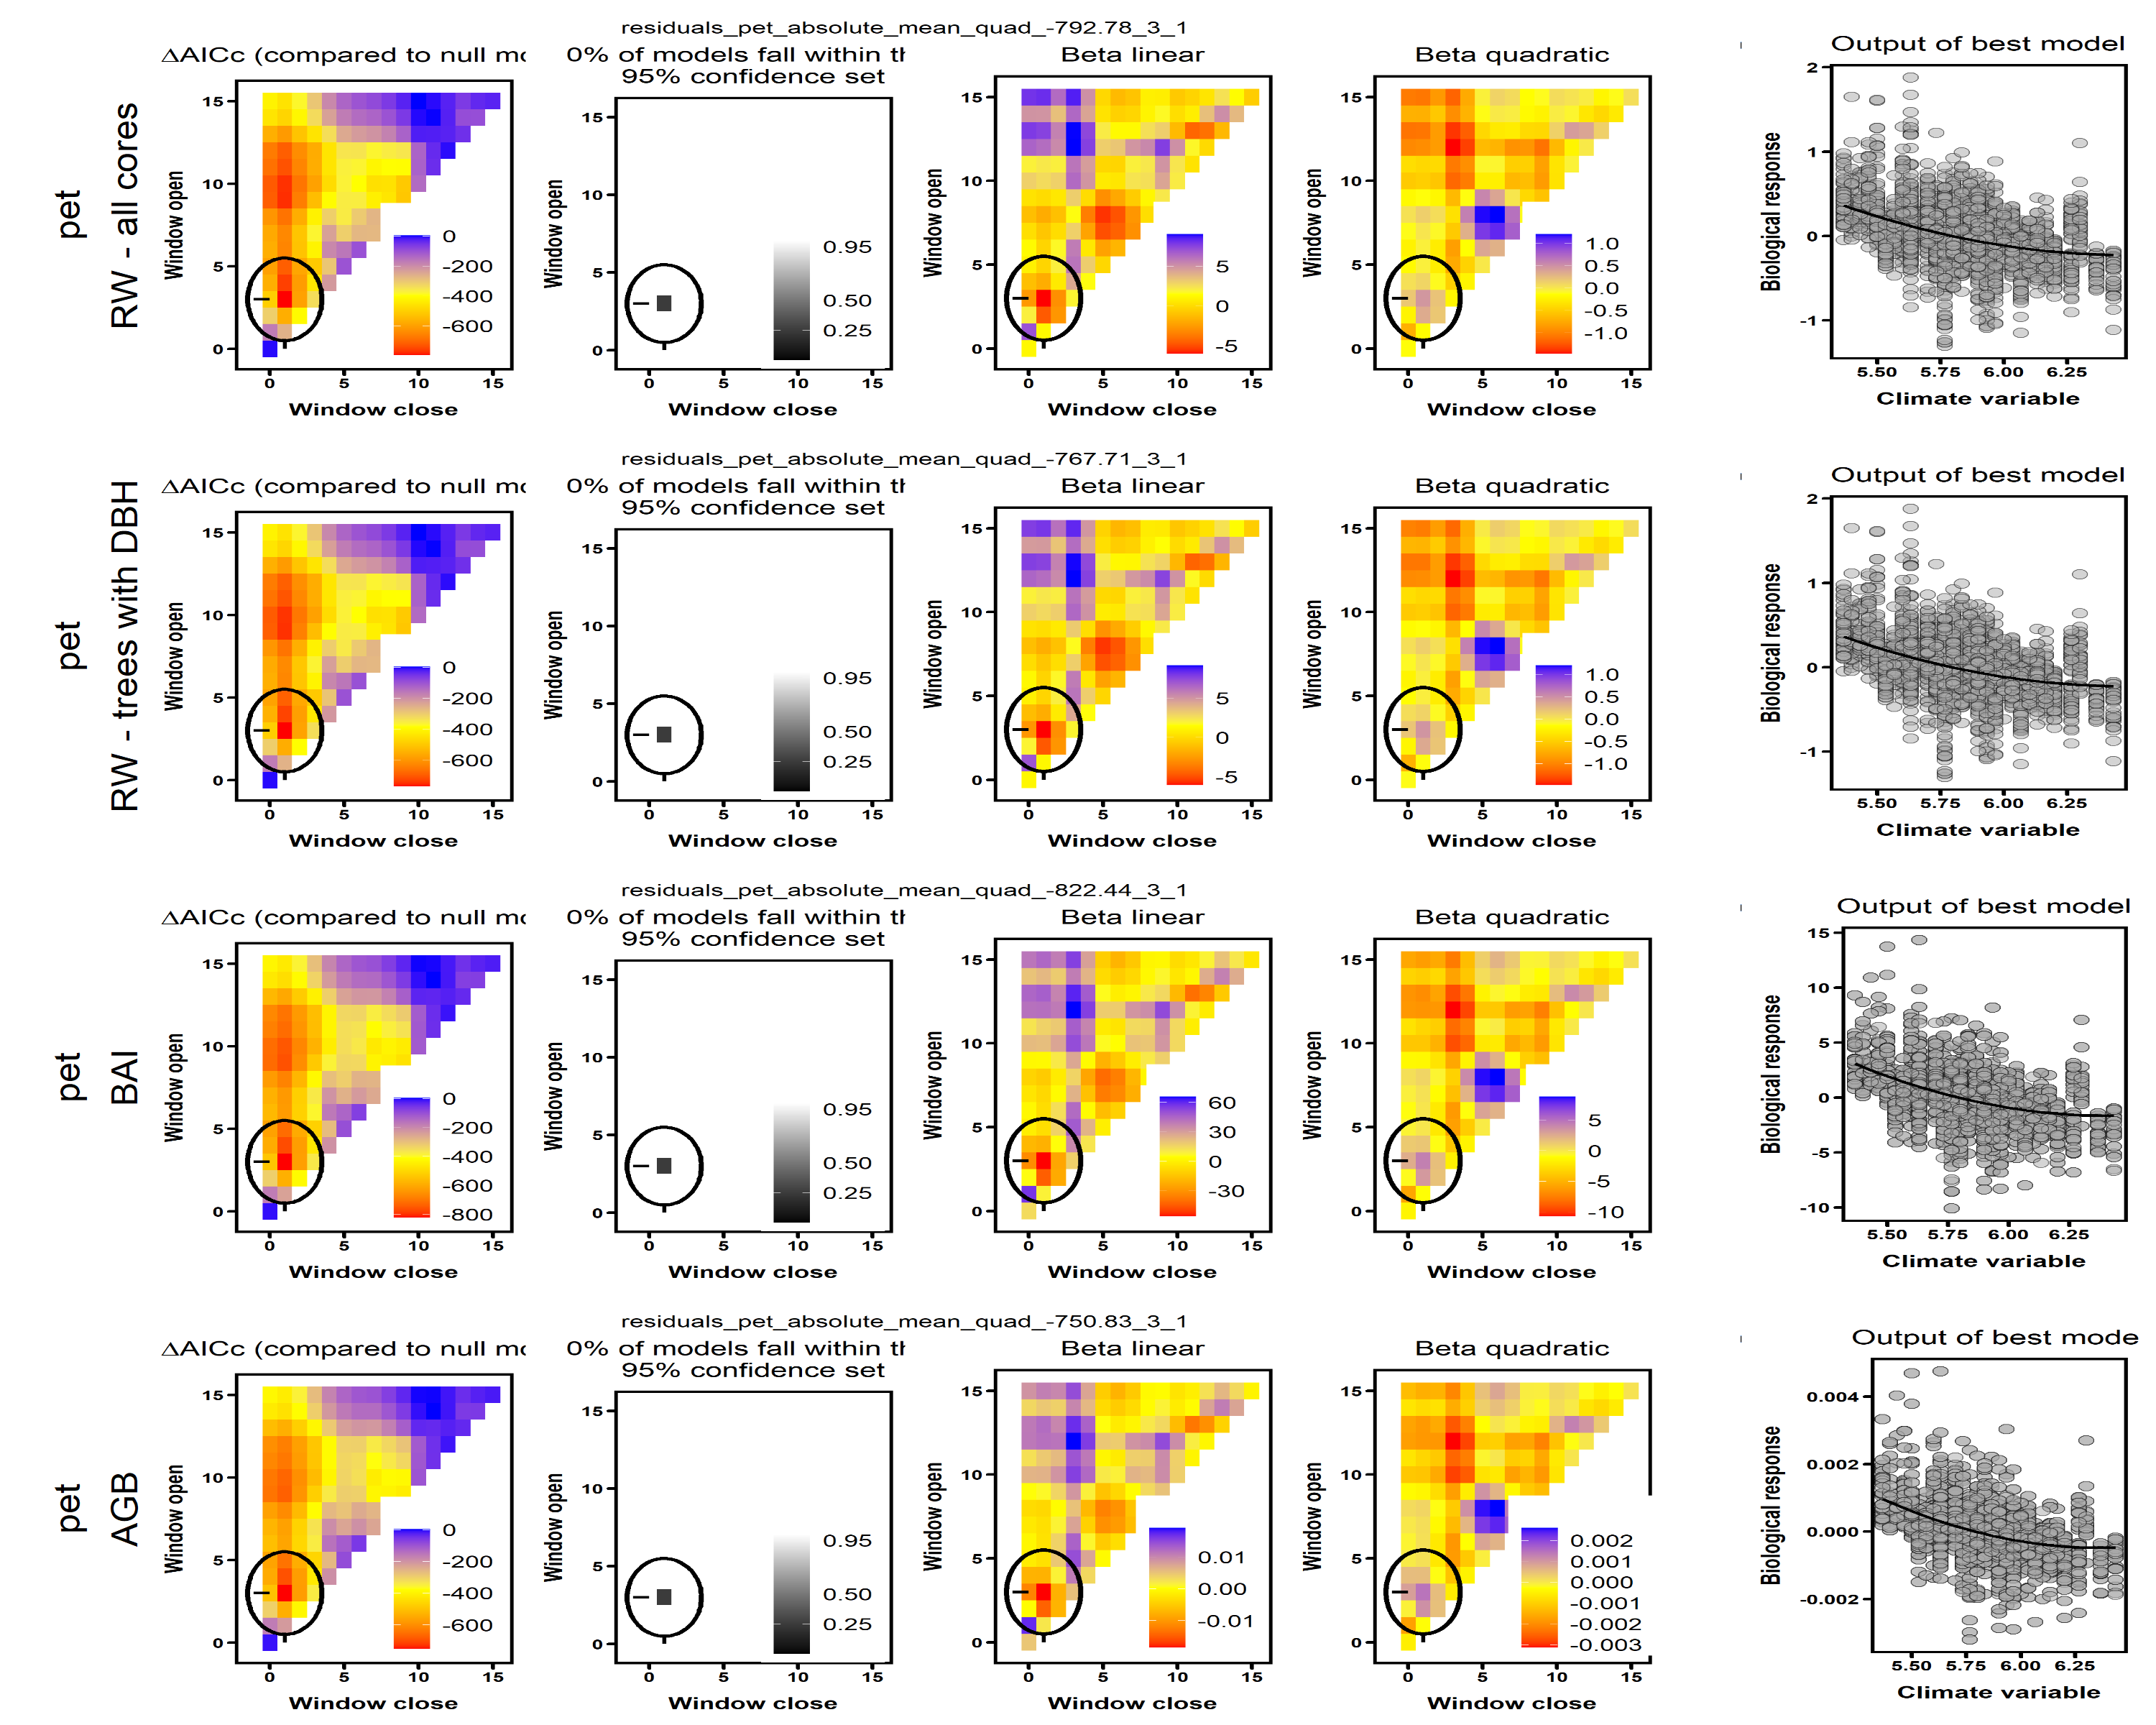
\includegraphics{/Users/kteixeira/Dropbox (Smithsonian)/GitHub/EcoClimLab/ForestGEO-climate-sensitivity/results/climwin_plots_combined/NewMexico_pet.png}
\caption{\textbf{Figure S2 \textbar{} Comparison of climwin output
across growth metrics for the temperature variable group at Little
Tesuque (New Mexico, USA).} Here, \emph{climwin} identified potential
evapotranspiration (\(PET\)) as the strongest climate variable across
all three metrics of growth (\(\Delta r\), BAI, \(\Delta AGB\)) and
regardless of whether all cores were included in the analysis, or only
those for which DBH could be reconstructed (\(\Delta r\)-trees with
\(DBH\), BAI, \(\Delta AGB\)).)}
\end{figure}

\newpage

\hypertarget{figure-s3.-comparison-of-climwin-output-across-growth-metrics-for-the-precipitation-variable-group-at-little-tesuque-new-mexico-usa}{%
\subsection{Figure S3. Comparison of climwin output across growth
metrics for the precipitation variable group at Little Tesuque (New
Mexico,
USA)}\label{figure-s3.-comparison-of-climwin-output-across-growth-metrics-for-the-precipitation-variable-group-at-little-tesuque-new-mexico-usa}}

\begin{figure}
\centering
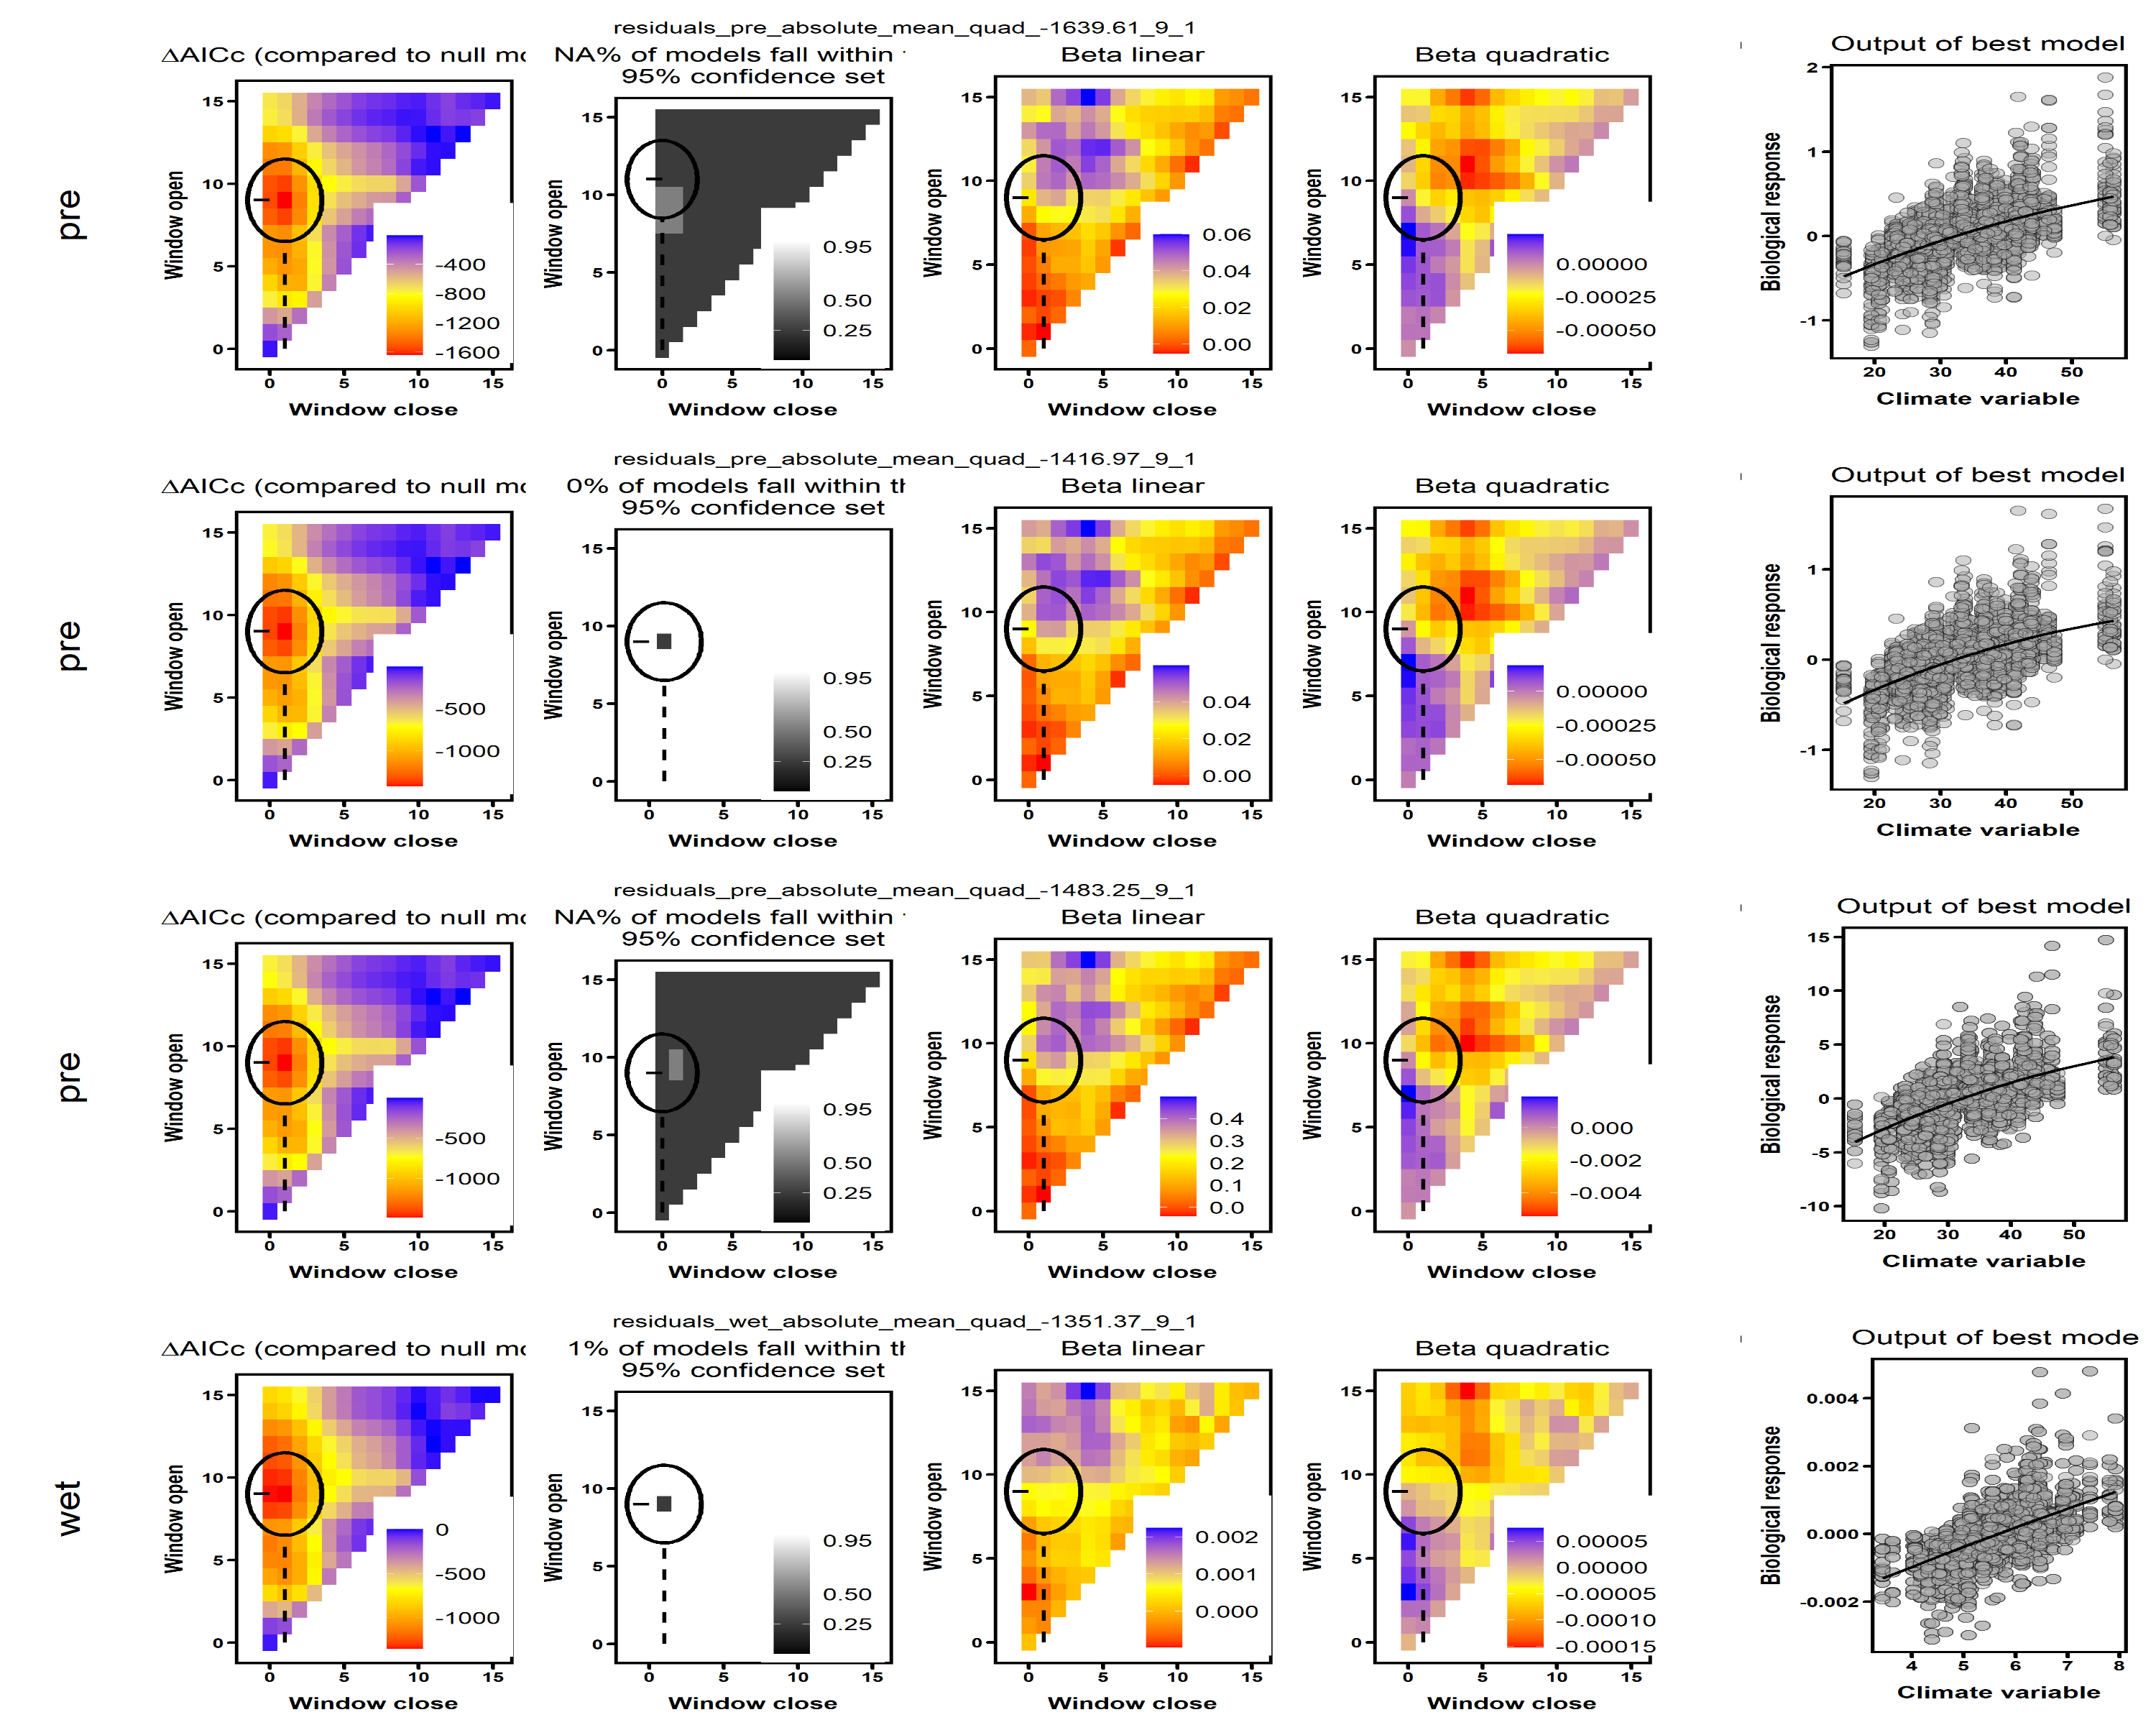
\includegraphics{/Users/kteixeira/Dropbox (Smithsonian)/GitHub/EcoClimLab/ForestGEO-climate-sensitivity/results/climwin_plots_combined/NewMexico_wet_pre.png}
\caption{\textbf{Figure S3 \textbar{} Comparison of climwin output
across growth metrics for the precipitation variable group at Little
Tesuque (New Mexico, USA).} Here, \emph{climwin} identified
precipitation (PRE) as the strongest climate variable for \(\Delta r\)
and \(BAI\), but precipitation day frequency (WET) as the strongest
climate variable for \(\Delta AGB\).}
\end{figure}

\newpage

\hypertarget{figure-s4.-comparison-of-climwin-output-across-growth-metrics-for-the-precipitation-variable-group-at-harvard-forest-massachusetts-usa}{%
\subsection{Figure S4. Comparison of climwin output across growth
metrics for the precipitation variable group at Harvard Forest
(Massachusetts,
USA)}\label{figure-s4.-comparison-of-climwin-output-across-growth-metrics-for-the-precipitation-variable-group-at-harvard-forest-massachusetts-usa}}

\begin{figure}
\centering
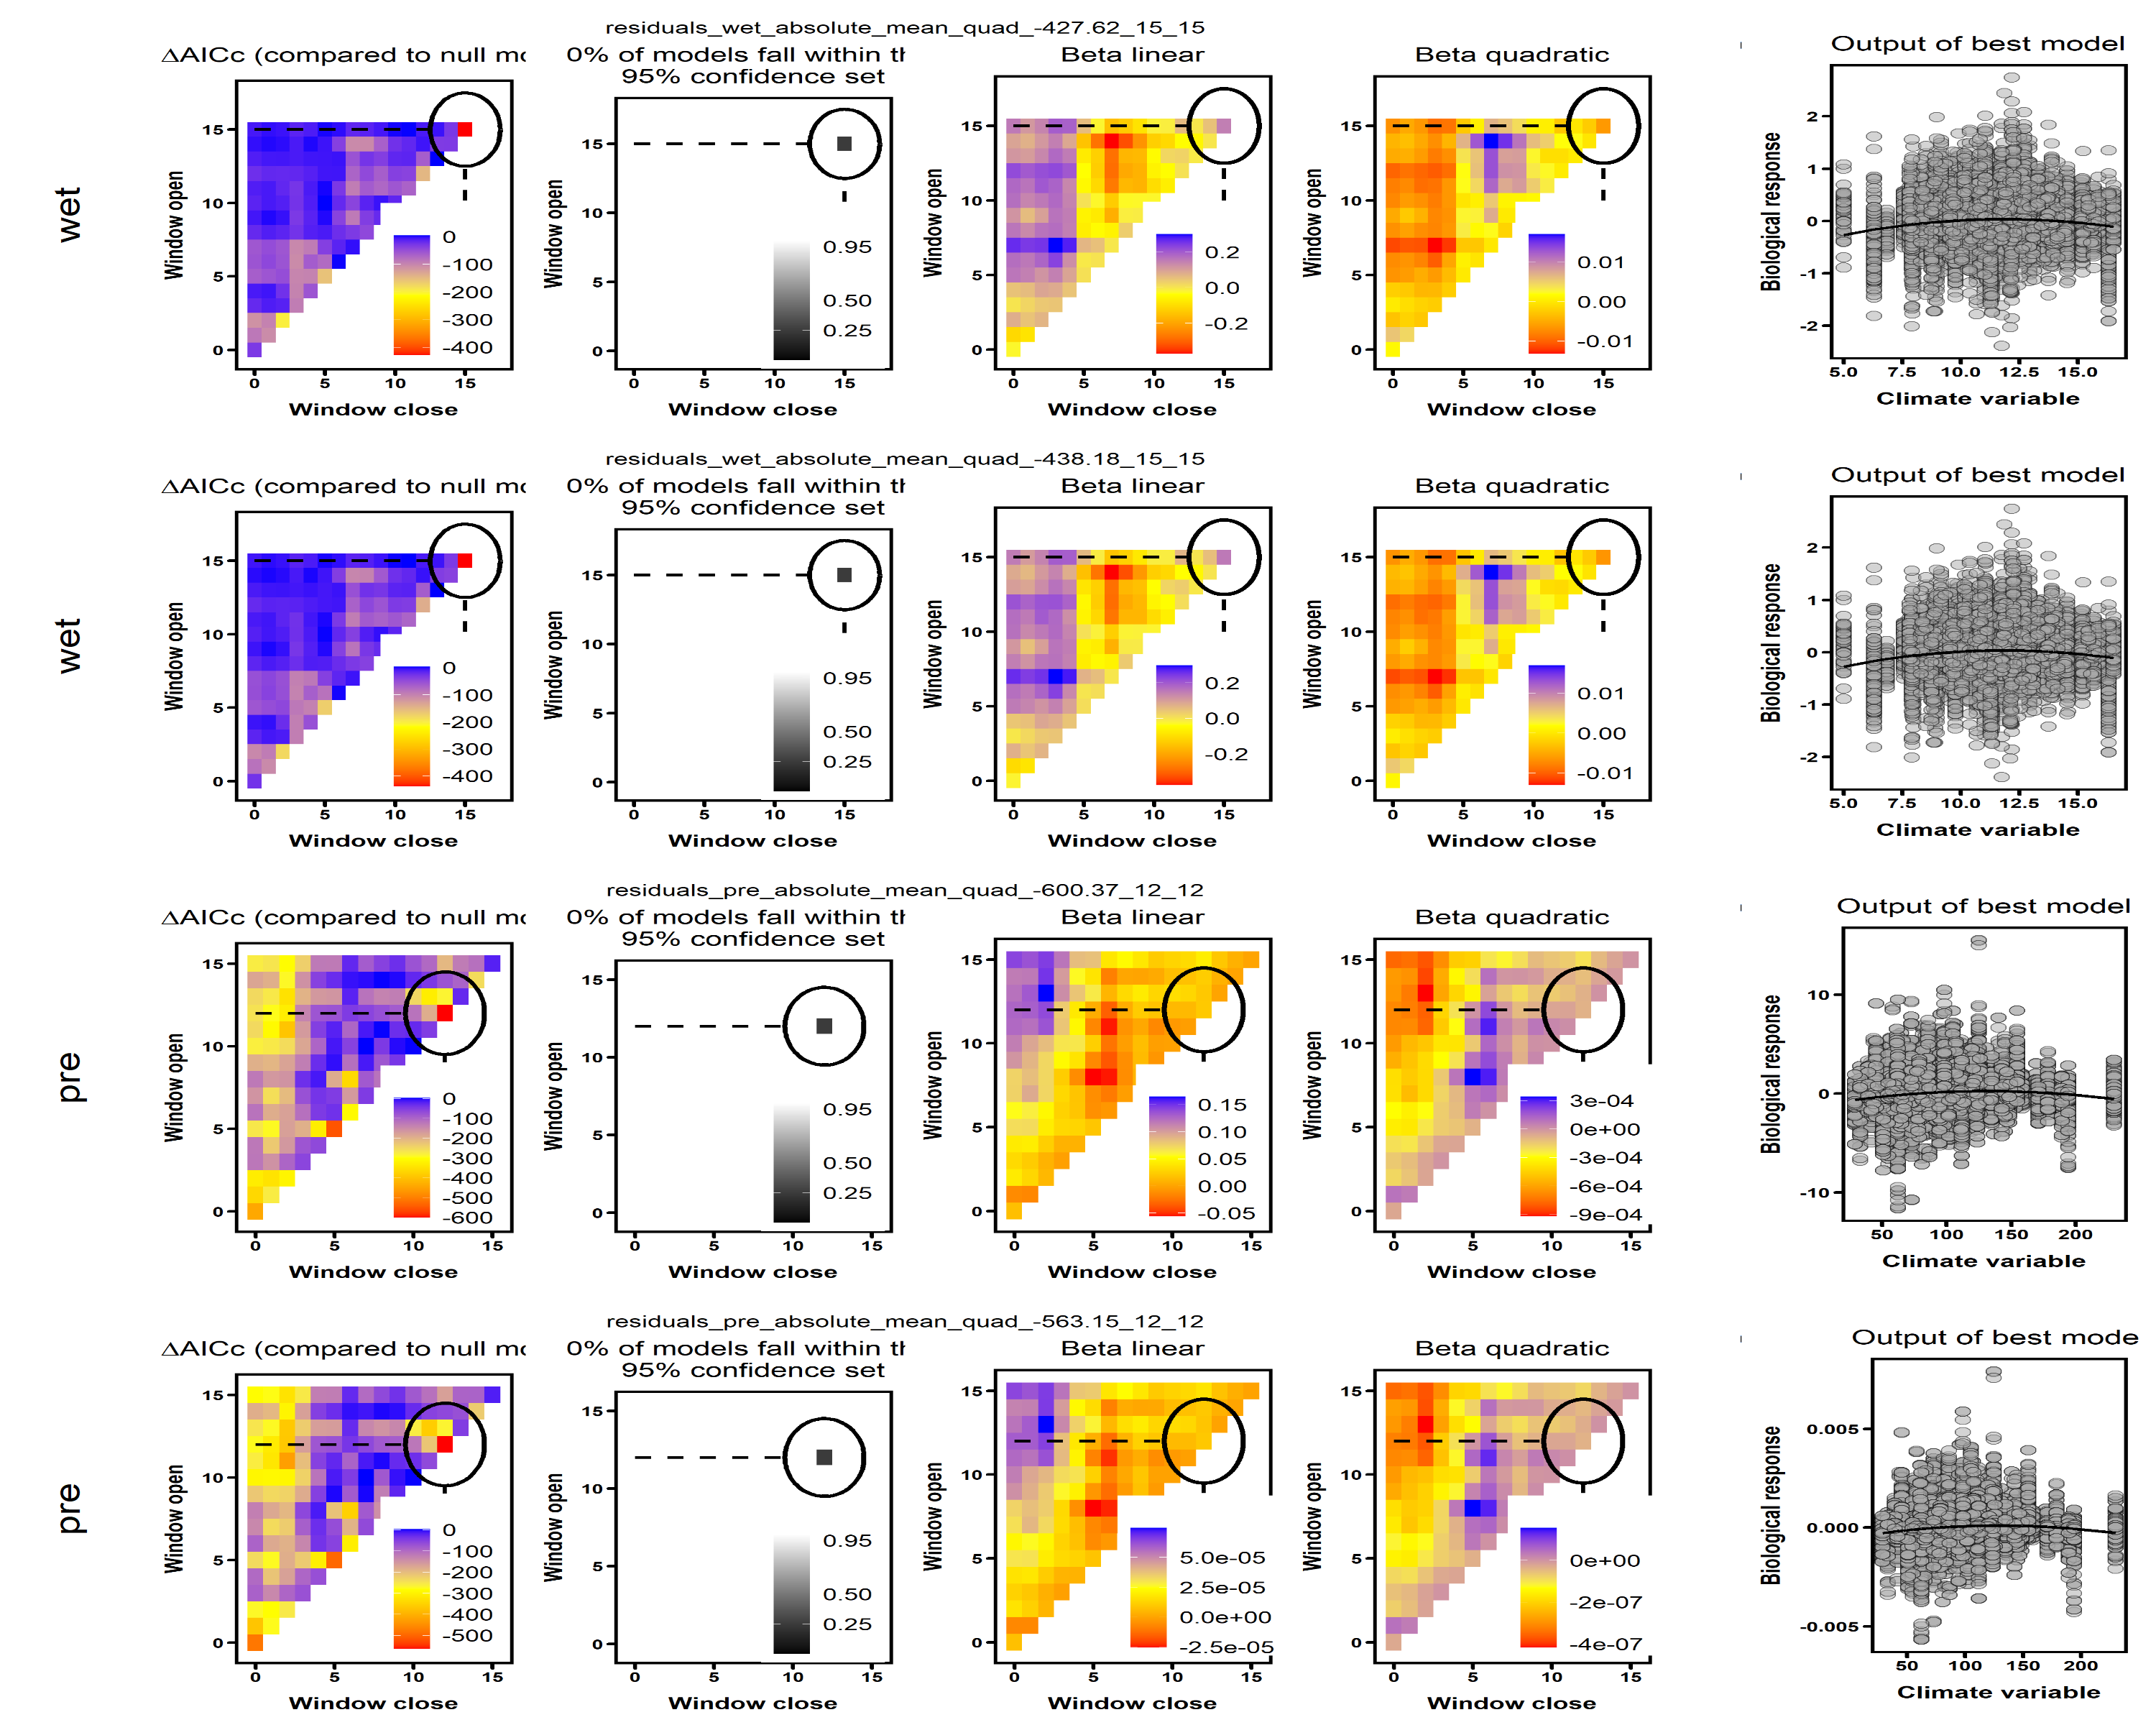
\includegraphics{/Users/kteixeira/Dropbox (Smithsonian)/GitHub/EcoClimLab/ForestGEO-climate-sensitivity/results/climwin_plots_combined/HarvardForest_pre_wet.png}
\caption{\textbf{Figure S4 \textbar{} Comparison of climwin output
across growth metrics for the precipitation variable group at Harvard
Forest (Massachusetts, USA).} Here, \emph{climwin} identified
precipitation frequency (WET) as the strongest climate variable for
\(\Delta r\), but precipitation amount (PRE) as the strongest climate
variable for \(BAI\) and \(\Delta AGB\). The optimal time window
(circled) also differed across growth metrics.}
\end{figure}

\newpage

\hypertarget{figure-s5.-best-gls-models-for-barro-colorado-island-panama}{%
\subsection{Figure S5. Best GLS models for Barro Colorado Island
(Panama)}\label{figure-s5.-best-gls-models-for-barro-colorado-island-panama}}

\begin{figure}
\centering
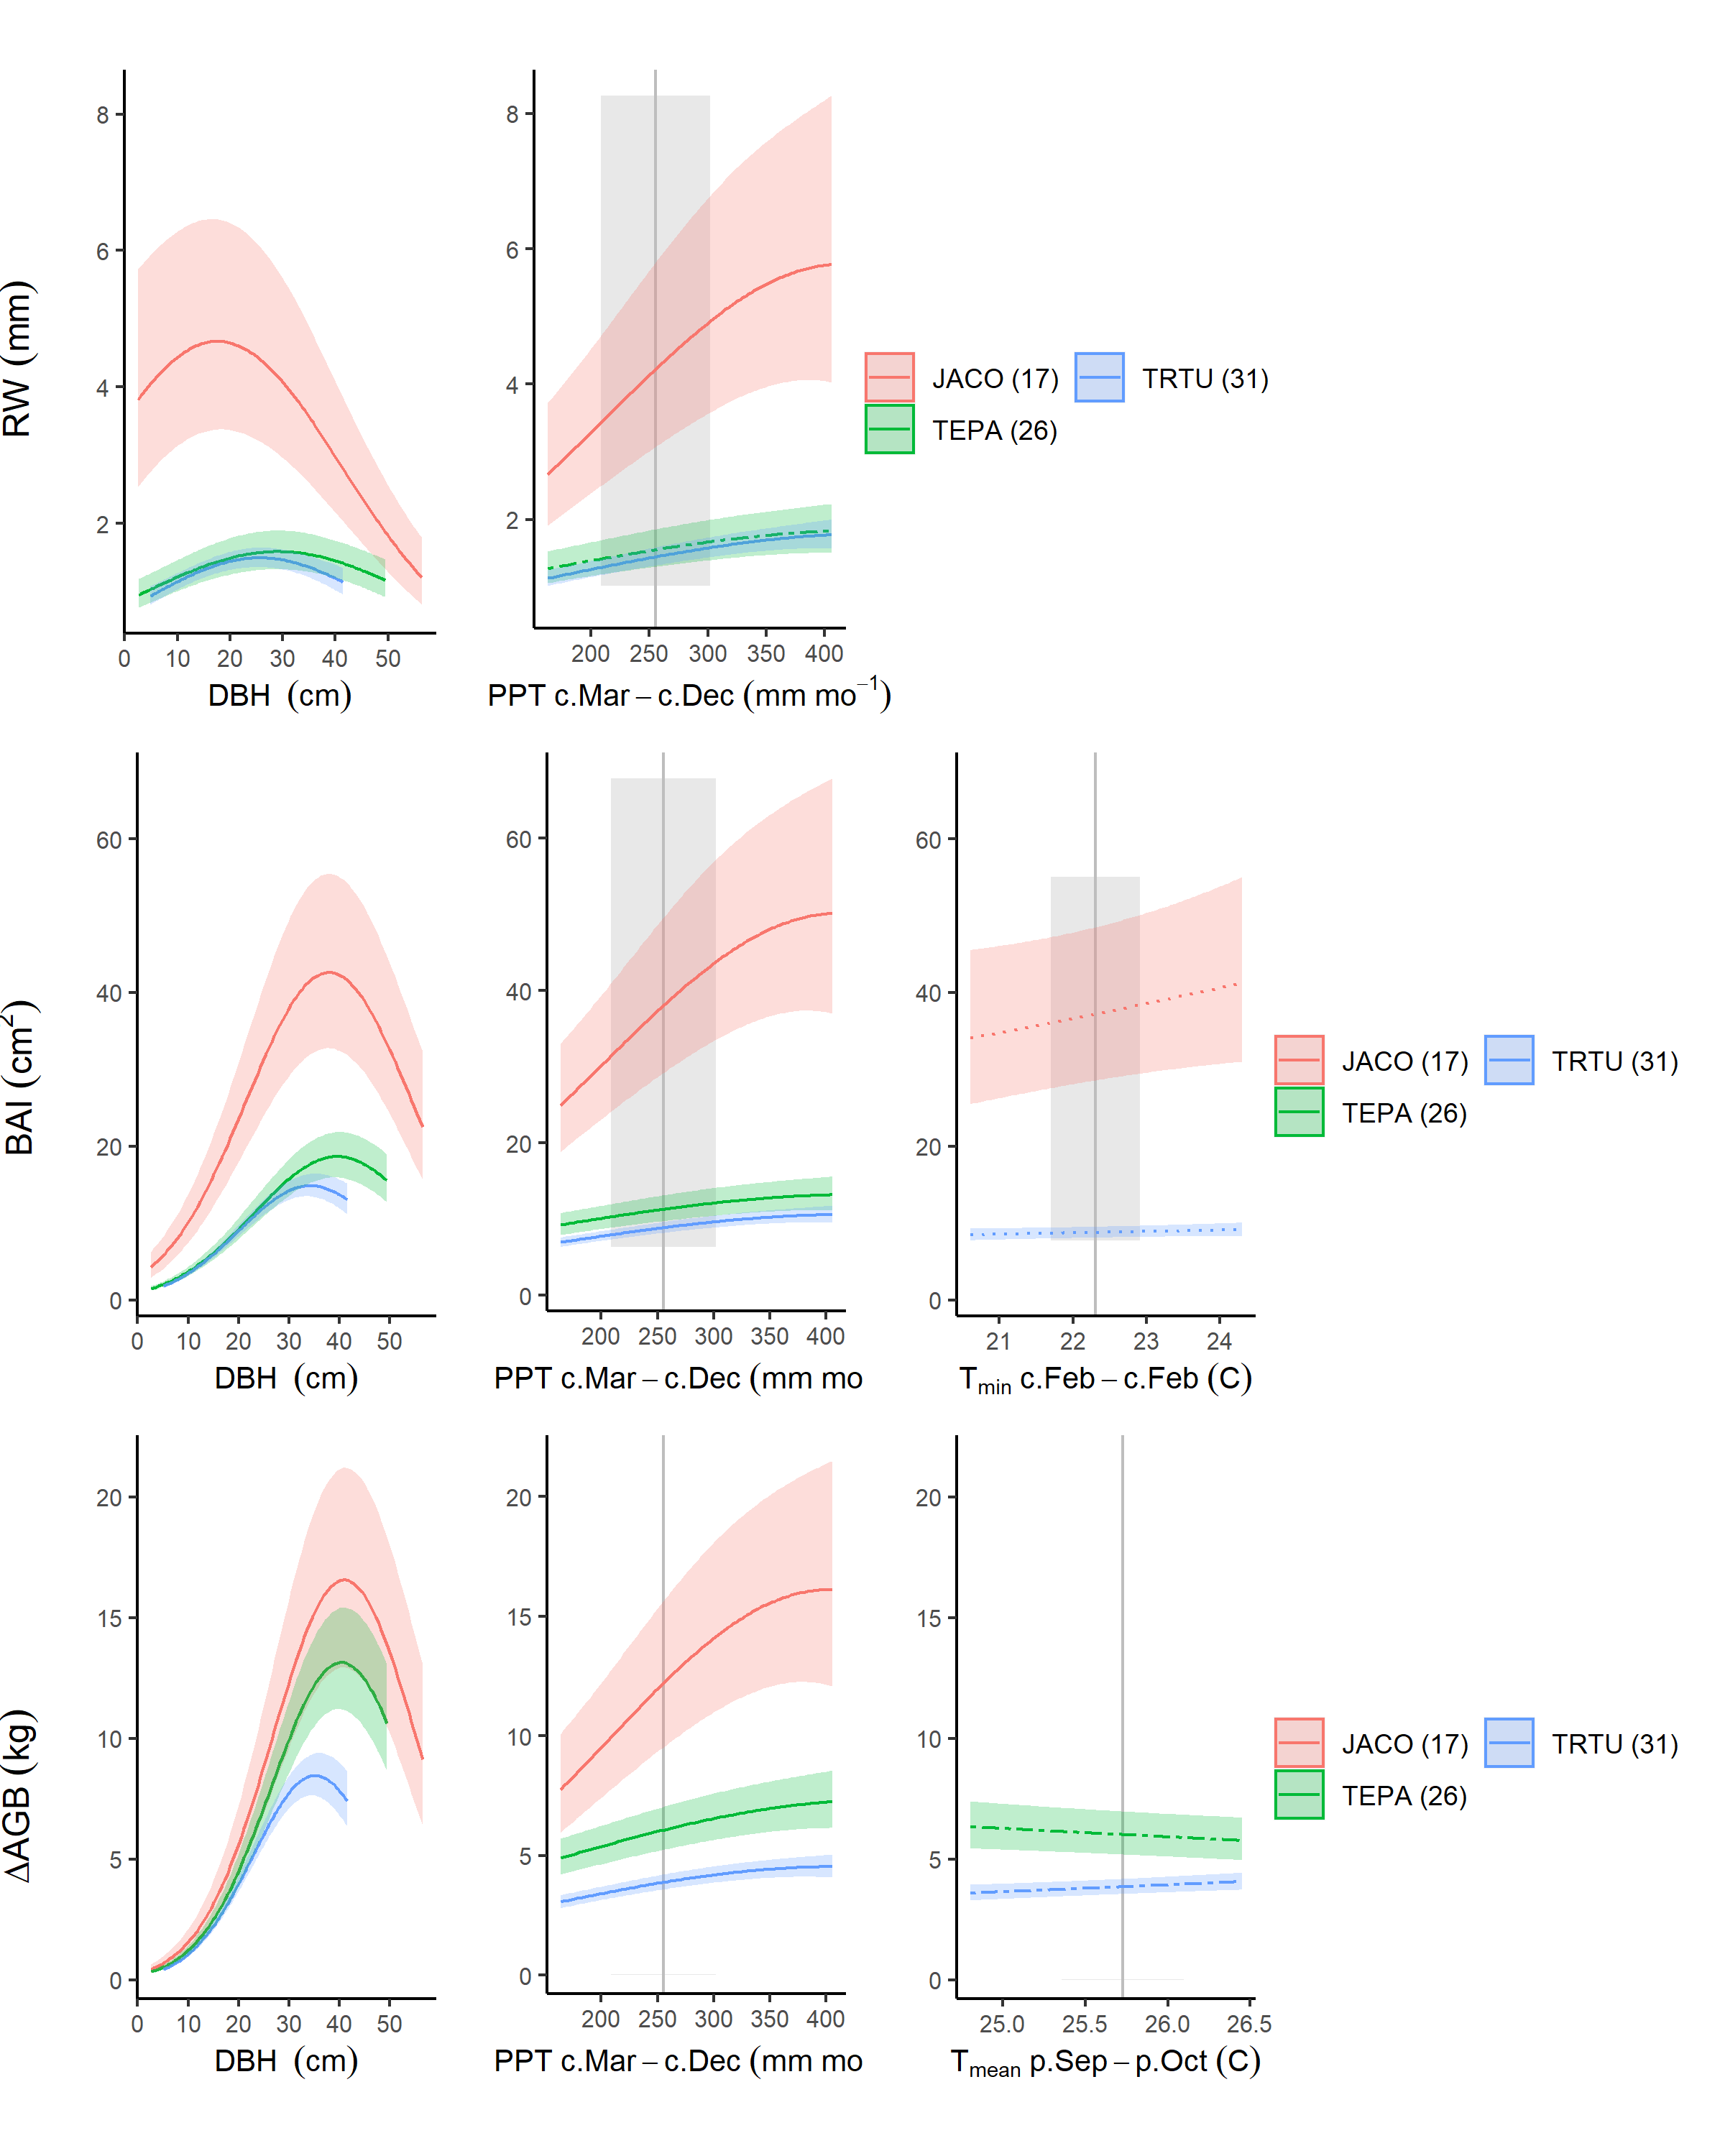
\includegraphics[width=0.78\textwidth,height=\textheight]{/Users/kteixeira/Dropbox (Smithsonian)/GitHub/EcoClimLab/ForestGEO-climate-sensitivity/results/composite_plots/BCI.png}
\caption{\textbf{Figure S5 \textbar{} Best GLS models for Barro Colorado
Island (Panama) for all three growth metrics: \(\Delta r\), \(BAI\), and
\(\Delta AGB\).} Precipitation and temperature group variables are as
selected by \emph{climwin}. For each species, relationships are plotted
if included in top model, with dashed lines indicating terms that do not
significantly improve the model (relative to a model without). Vertical
grey lines indicate the long-term mean for the climate variable, shading
indicates 1 SD.}
\end{figure}

\newpage

\hypertarget{figure-s6.-best-gls-models-for-huai-kha-khaeng-thailand}{%
\subsection{Figure S6. Best GLS models for Huai Kha Khaeng
(Thailand)}\label{figure-s6.-best-gls-models-for-huai-kha-khaeng-thailand}}

\begin{figure}
\centering
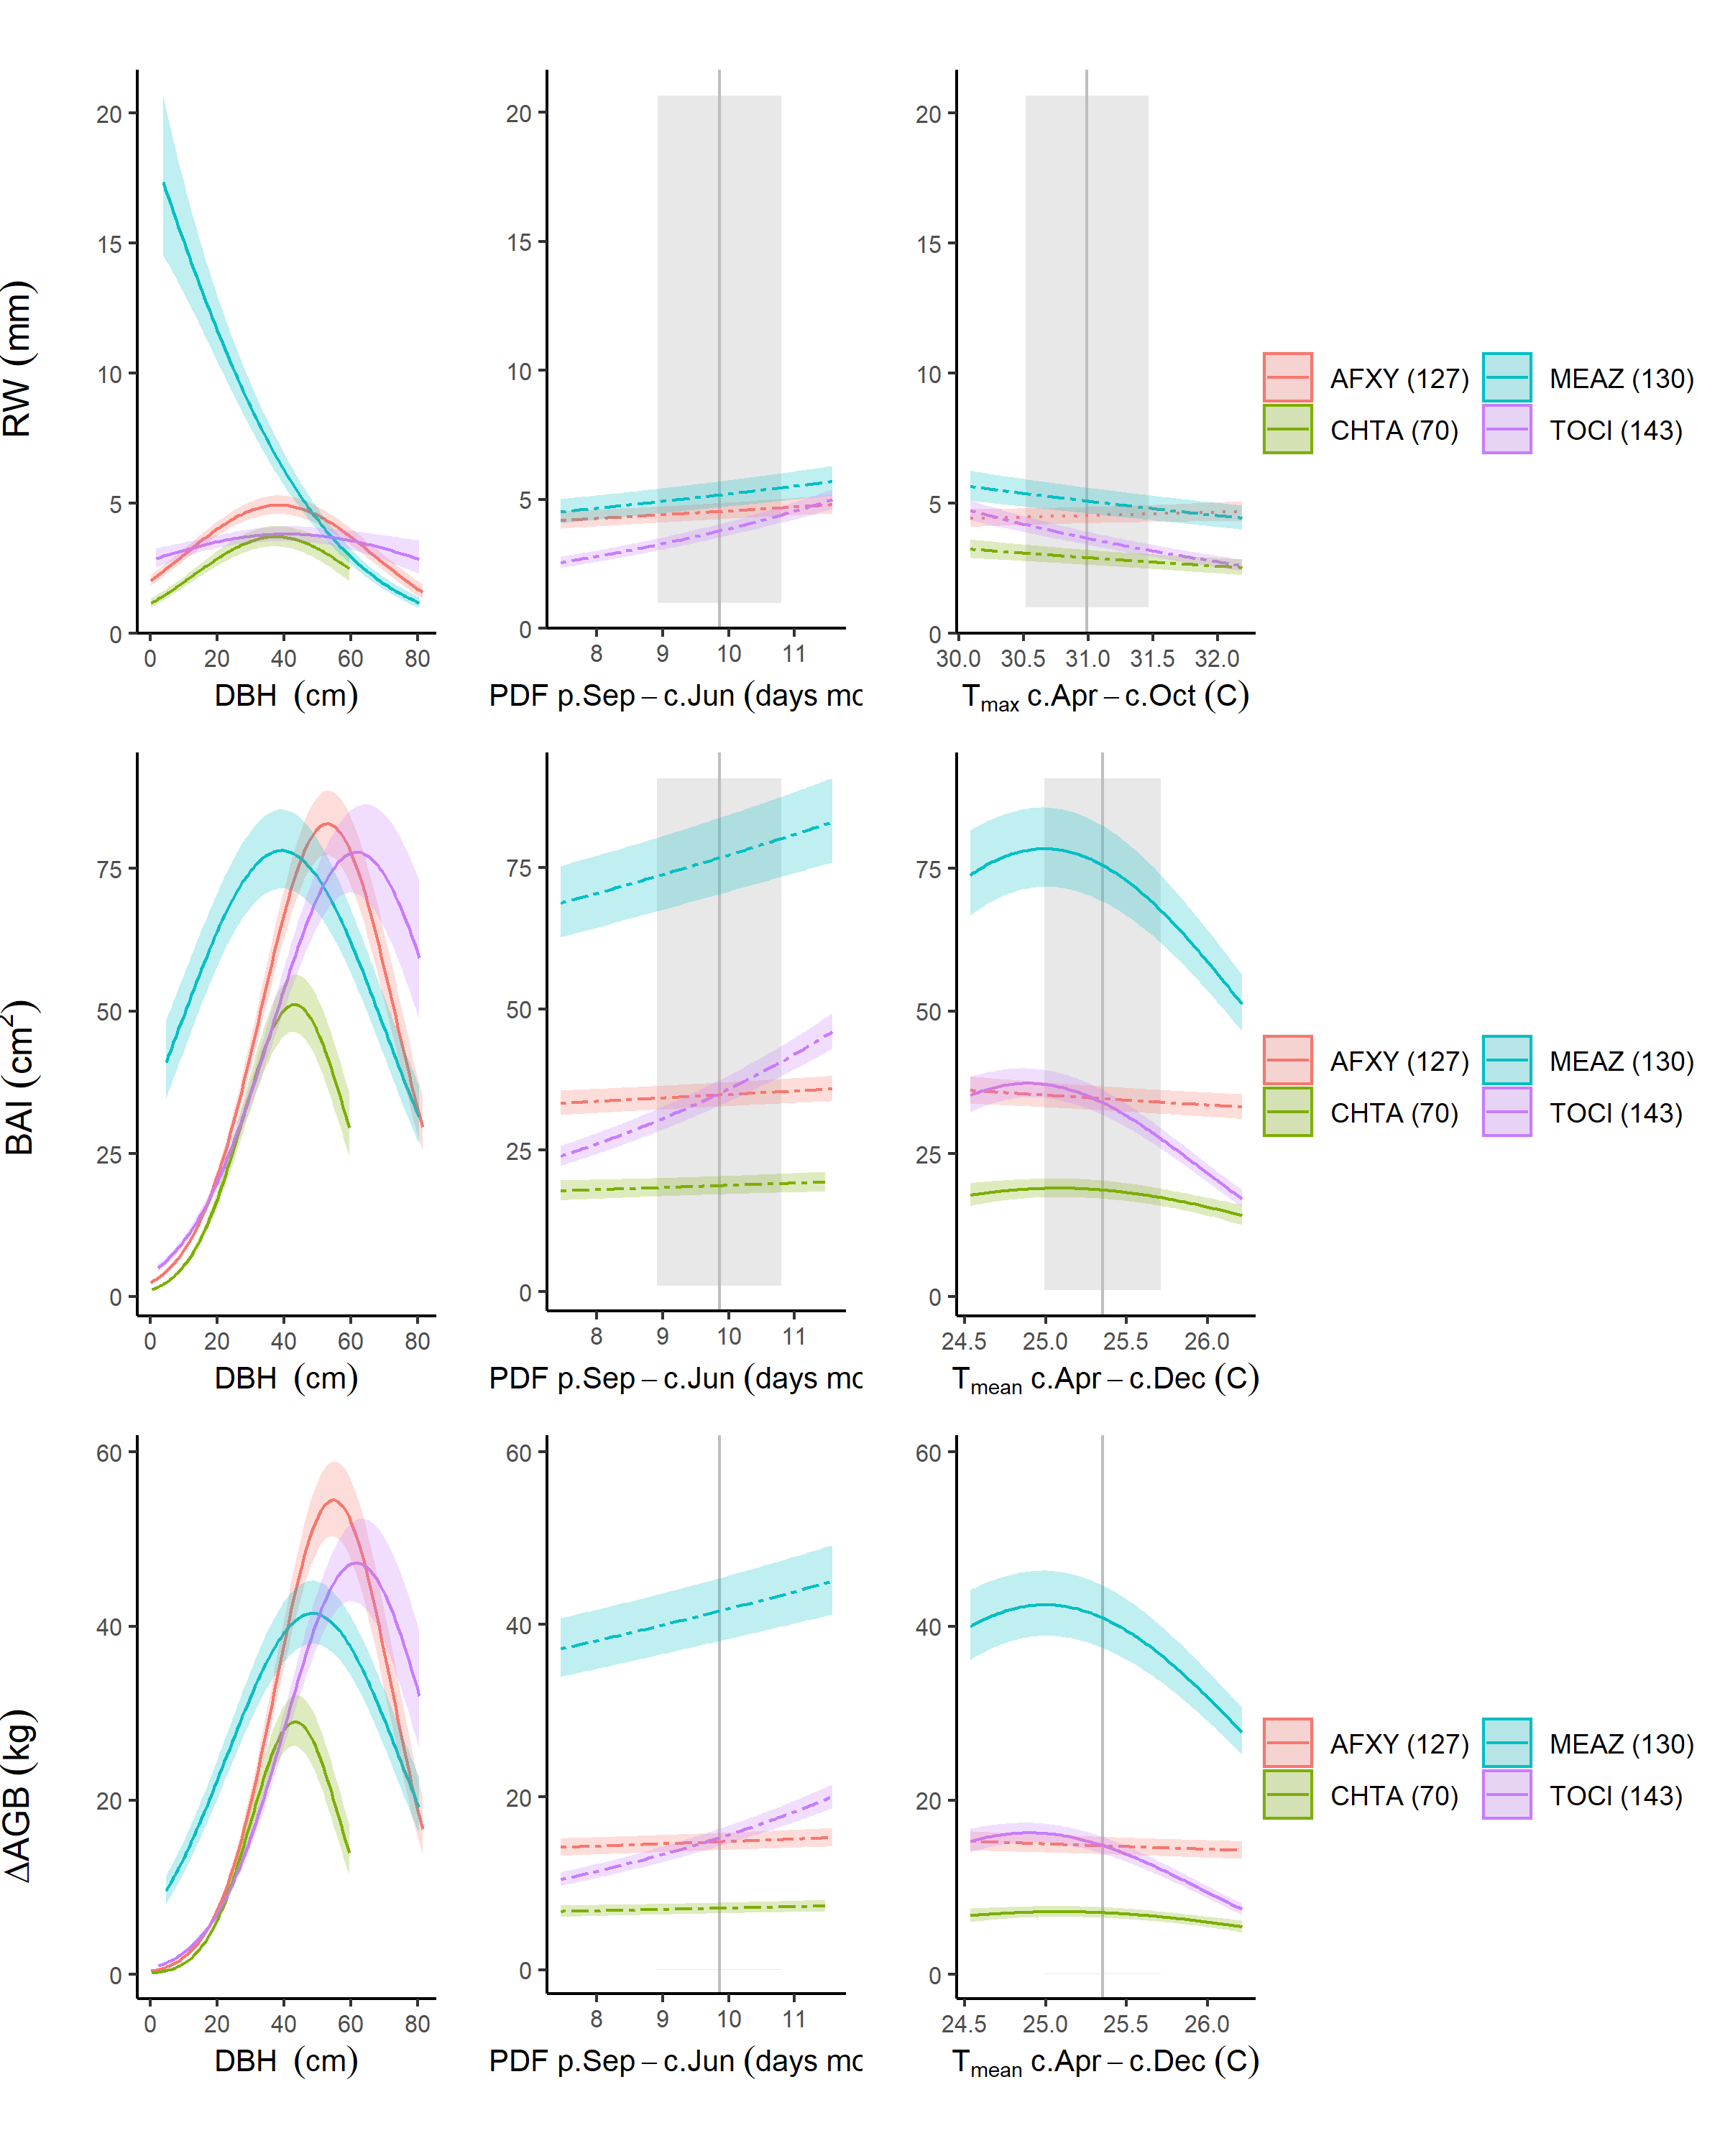
\includegraphics[width=0.78\textwidth,height=\textheight]{/Users/kteixeira/Dropbox (Smithsonian)/GitHub/EcoClimLab/ForestGEO-climate-sensitivity/results/composite_plots/HKK.png}
\caption{\textbf{Figure S6 \textbar{} Best GLS models for Huai Kha
Khaeng (Thailand) for all three growth metrics: \(\Delta r\), \(BAI\),
and \(\Delta AGB\).} Precipitation and temperature group variables are
as selected by \emph{climwin}. For each species, relationships are
plotted if included in top model, with dashed lines indicating terms
that do not significantly improve the model (relative to a model
without). Vertical grey lines indicate the long-term mean for the
climate variable, shading indicates 1 SD.}
\end{figure}

\newpage

\hypertarget{figure-s7.-best-gls-models-for-little-tesuque-new-mexico-usa}{%
\subsection{Figure S7. Best GLS models for Little Tesuque (New Mexico,
USA)}\label{figure-s7.-best-gls-models-for-little-tesuque-new-mexico-usa}}

\begin{figure}
\centering
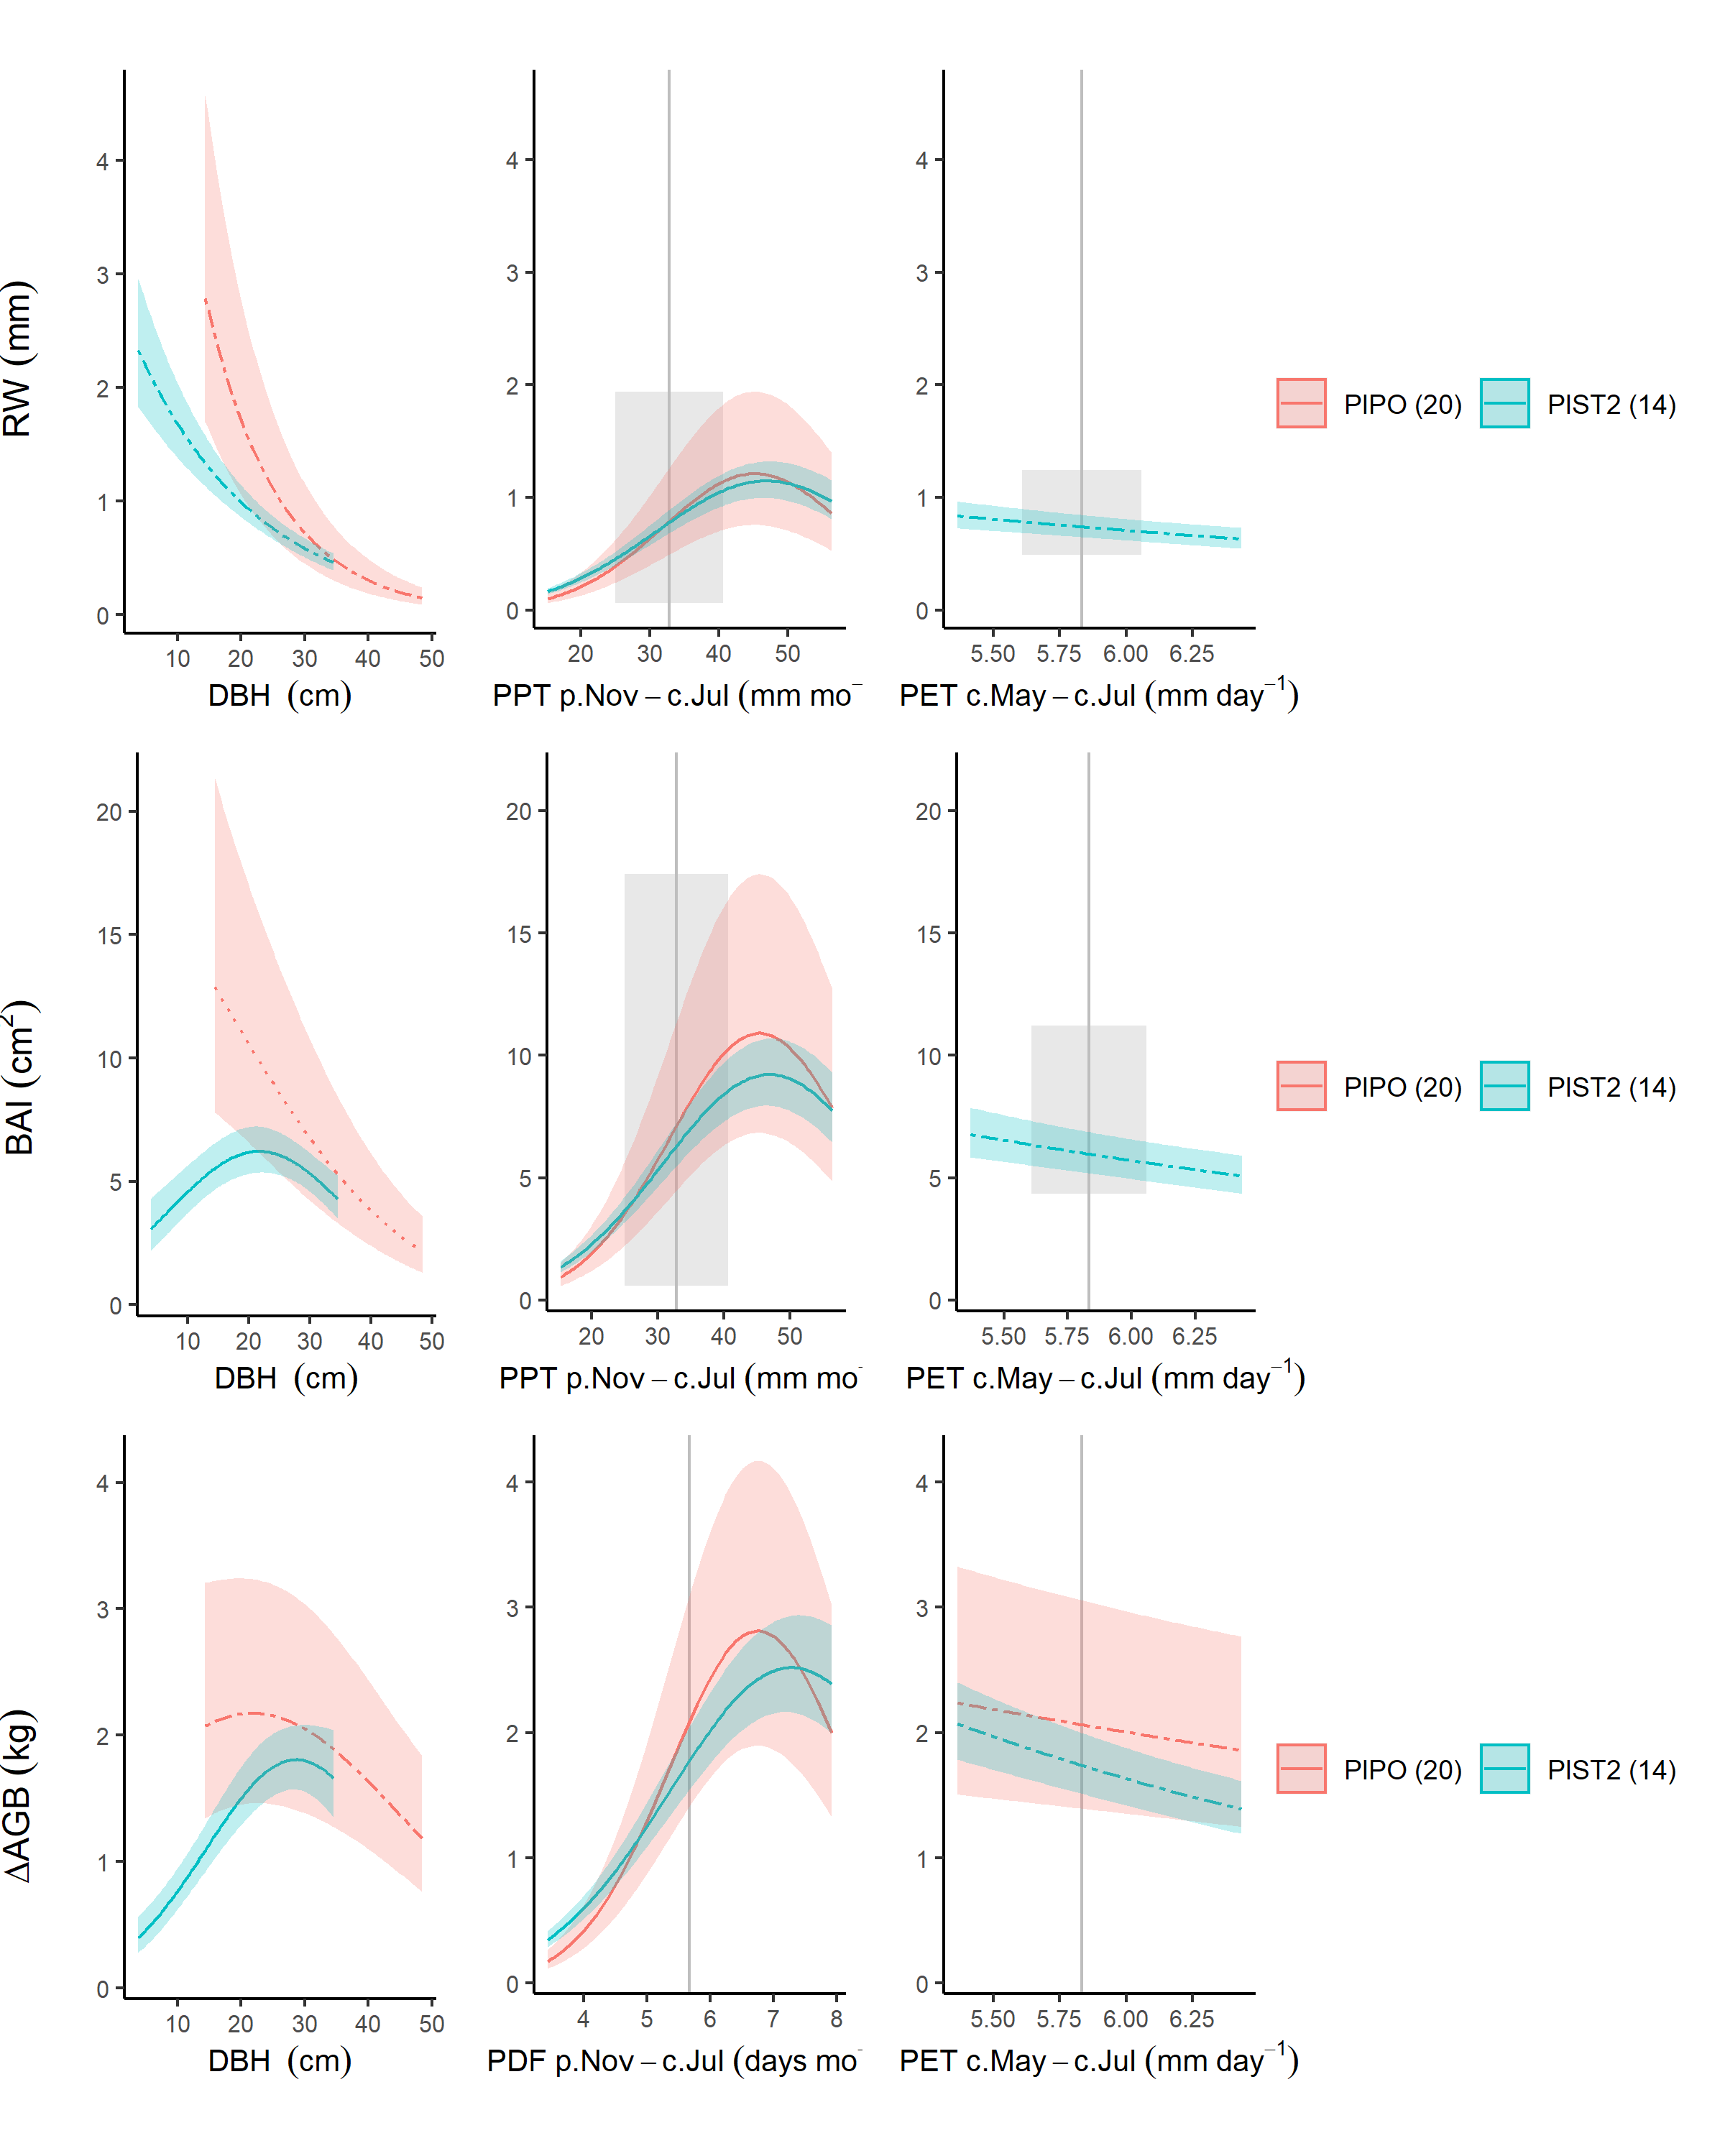
\includegraphics[width=0.78\textwidth,height=\textheight]{/Users/kteixeira/Dropbox (Smithsonian)/GitHub/EcoClimLab/ForestGEO-climate-sensitivity/results/composite_plots/NewMexico.png}
\caption{\textbf{Figure S7 \textbar{} Best GLS models for Little Tesuque
(New Mexico, USA) for all three growth metrics: \(\Delta r\), \(BAI\),
and \(\Delta AGB\).} Precipitation and temperature group variables are
as selected by \emph{climwin}. For each species, relationships are
plotted if included in top model, with dashed lines indicating terms
that do not significantly improve the model (relative to a model
without). Vertical grey lines indicate the long-term mean for the
climate variable, shading indicates 1 SD.}
\end{figure}

\newpage

\hypertarget{figure-s8.-best-gls-models-for-cedar-breaks-utah-usa}{%
\subsection{Figure S8. Best GLS models for Cedar Breaks (Utah,
USA)}\label{figure-s8.-best-gls-models-for-cedar-breaks-utah-usa}}

{[}\textbf{Figure S8 \textbar{} Best GLS models for Cedar Breaks (Utah,
USA) for all three growth metrics: \(\Delta r\), \(BAI\), and
\(\Delta AGB\).} Precipitation and temperature group variables are as
selected by \emph{climwin}. For each species, relationships are plotted
if included in top model, with dashed lines indicating terms that do not
significantly improve the model (relative to a model without). Vertical
grey lines indicate the long-term mean for the climate variable, shading
indicates 1 SD.{]}

\newpage

\hypertarget{figure-s9.-best-gls-models-for-scbi-virginia-usa}{%
\subsection{Figure S9. Best GLS models for SCBI (Virginia,
USA)}\label{figure-s9.-best-gls-models-for-scbi-virginia-usa}}

\begin{figure}
\centering
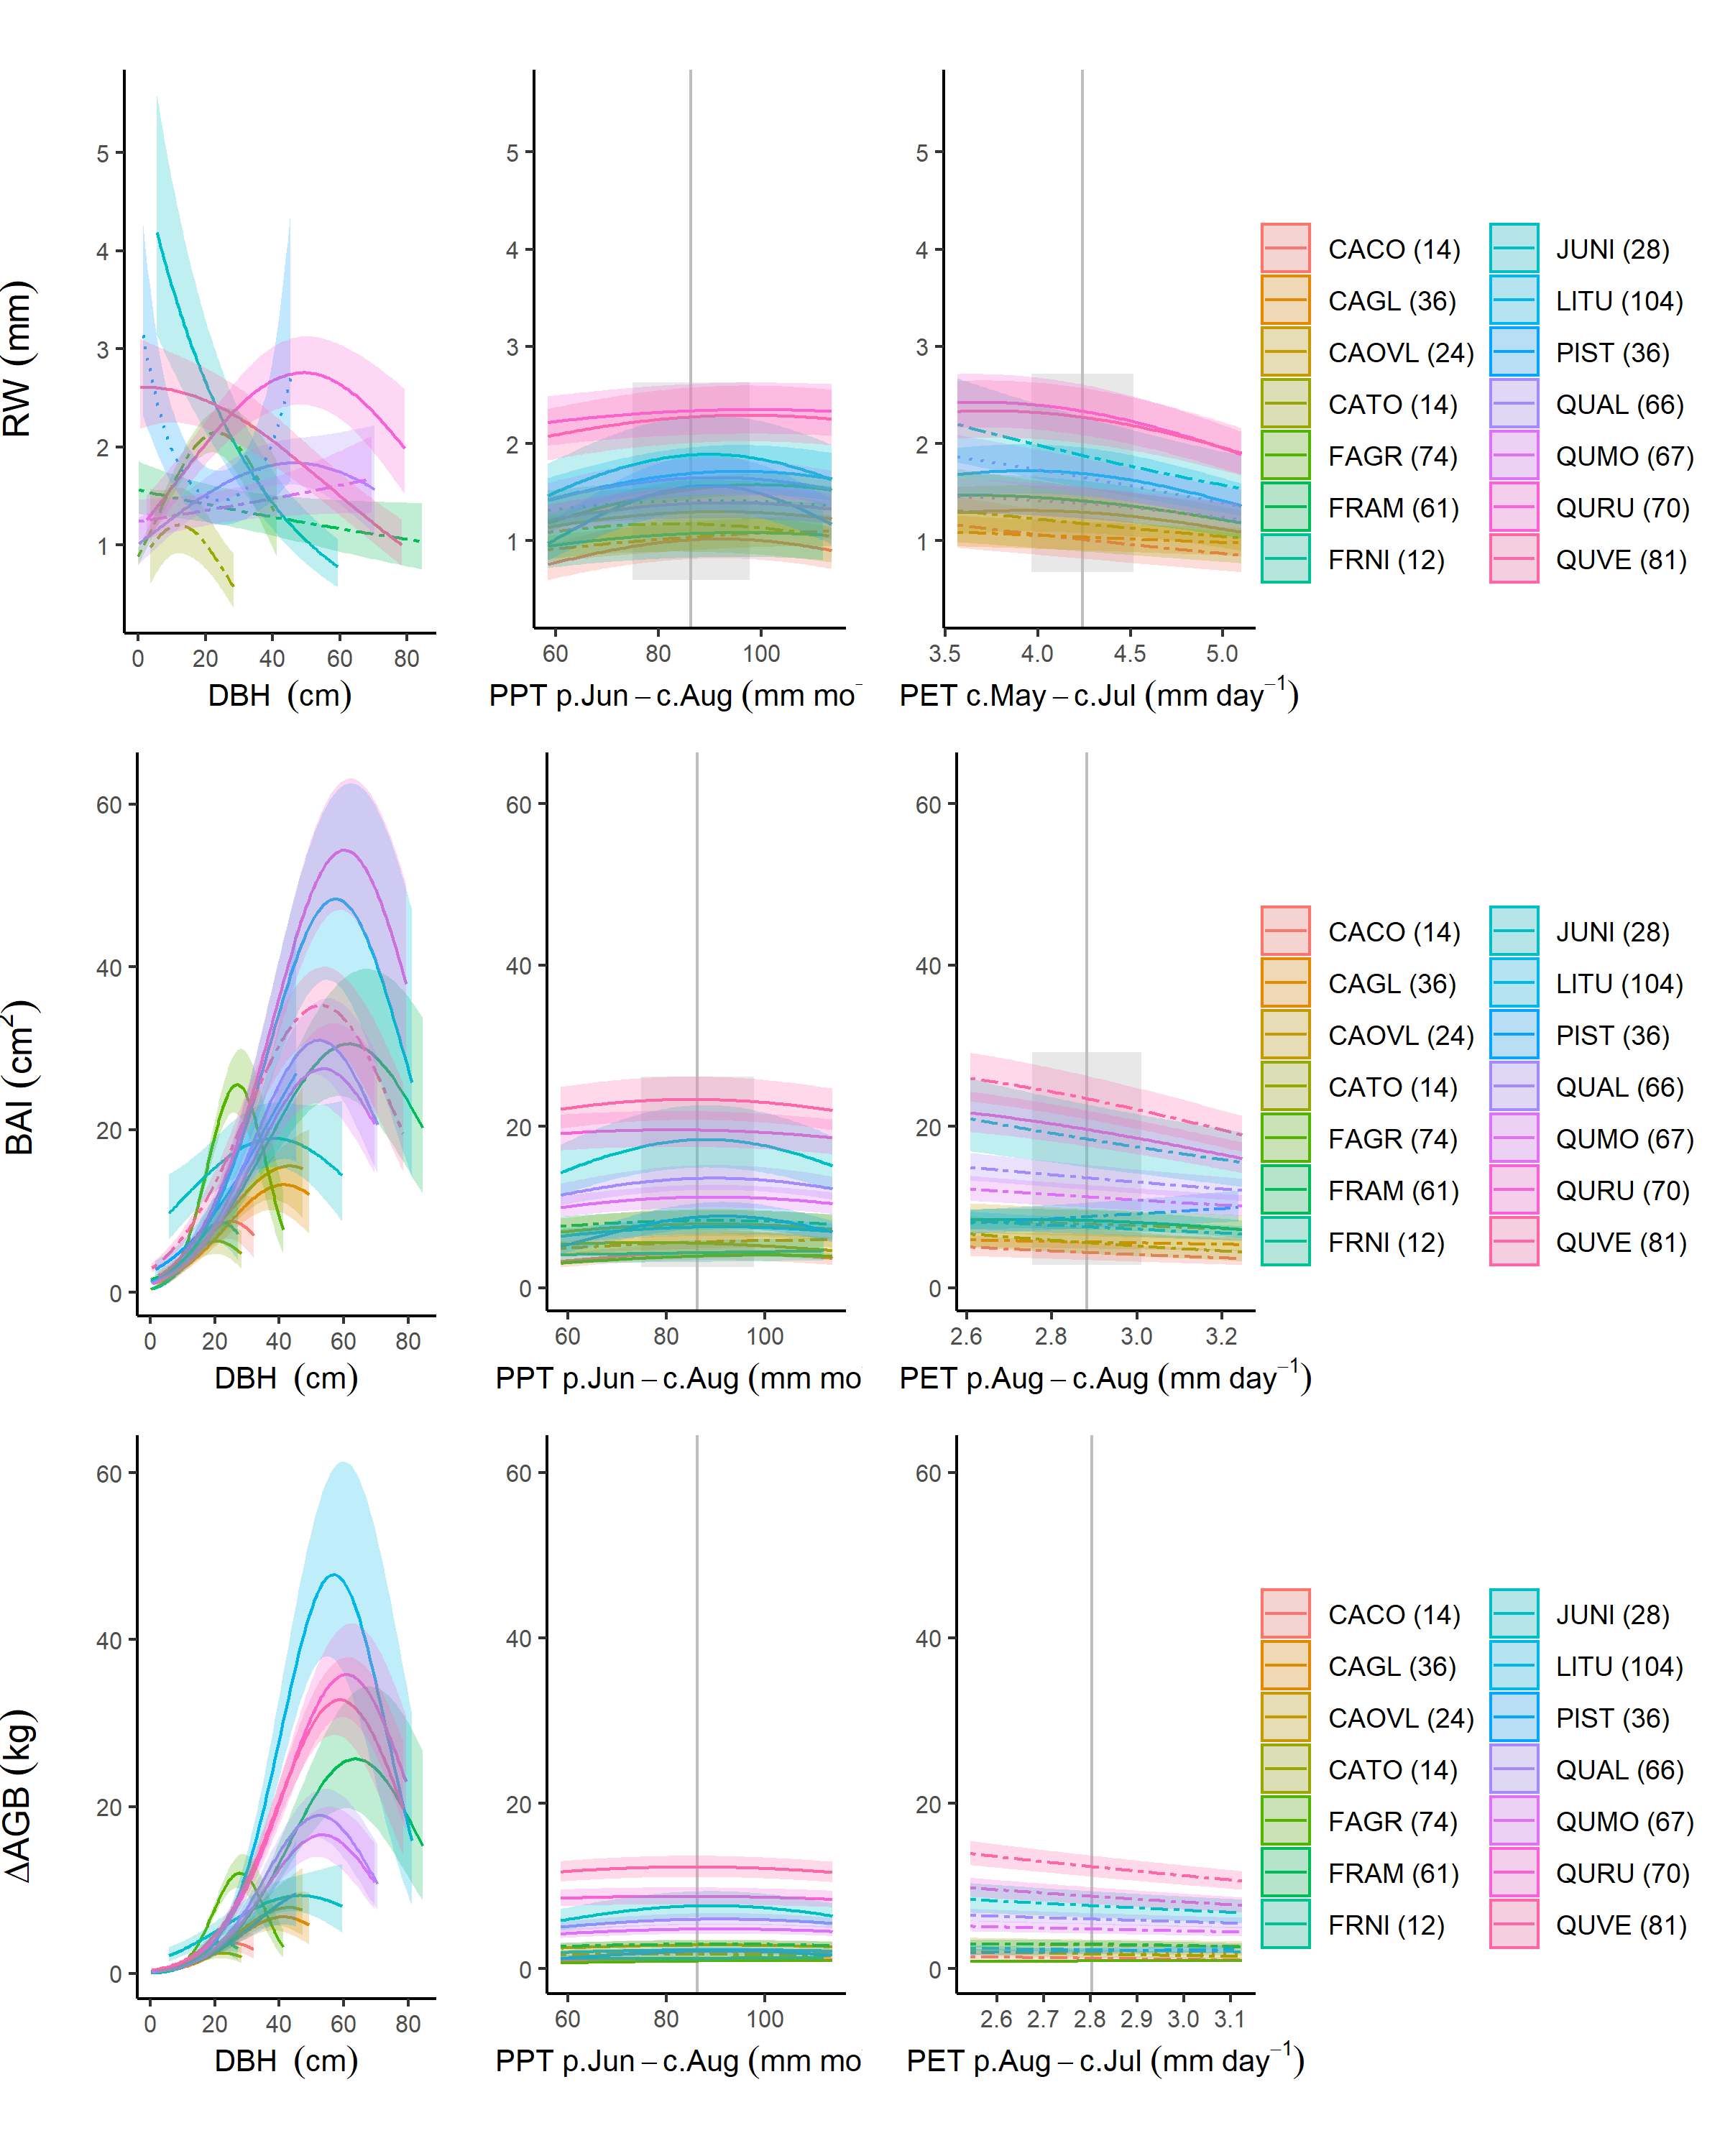
\includegraphics[width=0.78\textwidth,height=\textheight]{/Users/kteixeira/Dropbox (Smithsonian)/GitHub/EcoClimLab/ForestGEO-climate-sensitivity/results/composite_plots/SCBI.png}
\caption{\textbf{Figure S9 \textbar{} Best GLS models for SCBI
(Virginia, USA) for all three growth metrics: \(\Delta r\), \(BAI\), and
\(\Delta AGB\).} Precipitation and temperature group variables are as
selected by \emph{climwin}. For each species, relationships are plotted
if included in top model, with dashed lines indicating terms that do not
significantly improve the model (relative to a model without). Vertical
grey lines indicate the long-term mean for the climate variable, shading
indicates 1 SD.}
\end{figure}

\newpage

\hypertarget{figure-s10.-best-gls-models-for-lilly-dickey-woods-indiana-usa}{%
\subsection{Figure S10. Best GLS models for Lilly Dickey Woods (Indiana,
USA)}\label{figure-s10.-best-gls-models-for-lilly-dickey-woods-indiana-usa}}

\begin{figure}
\centering
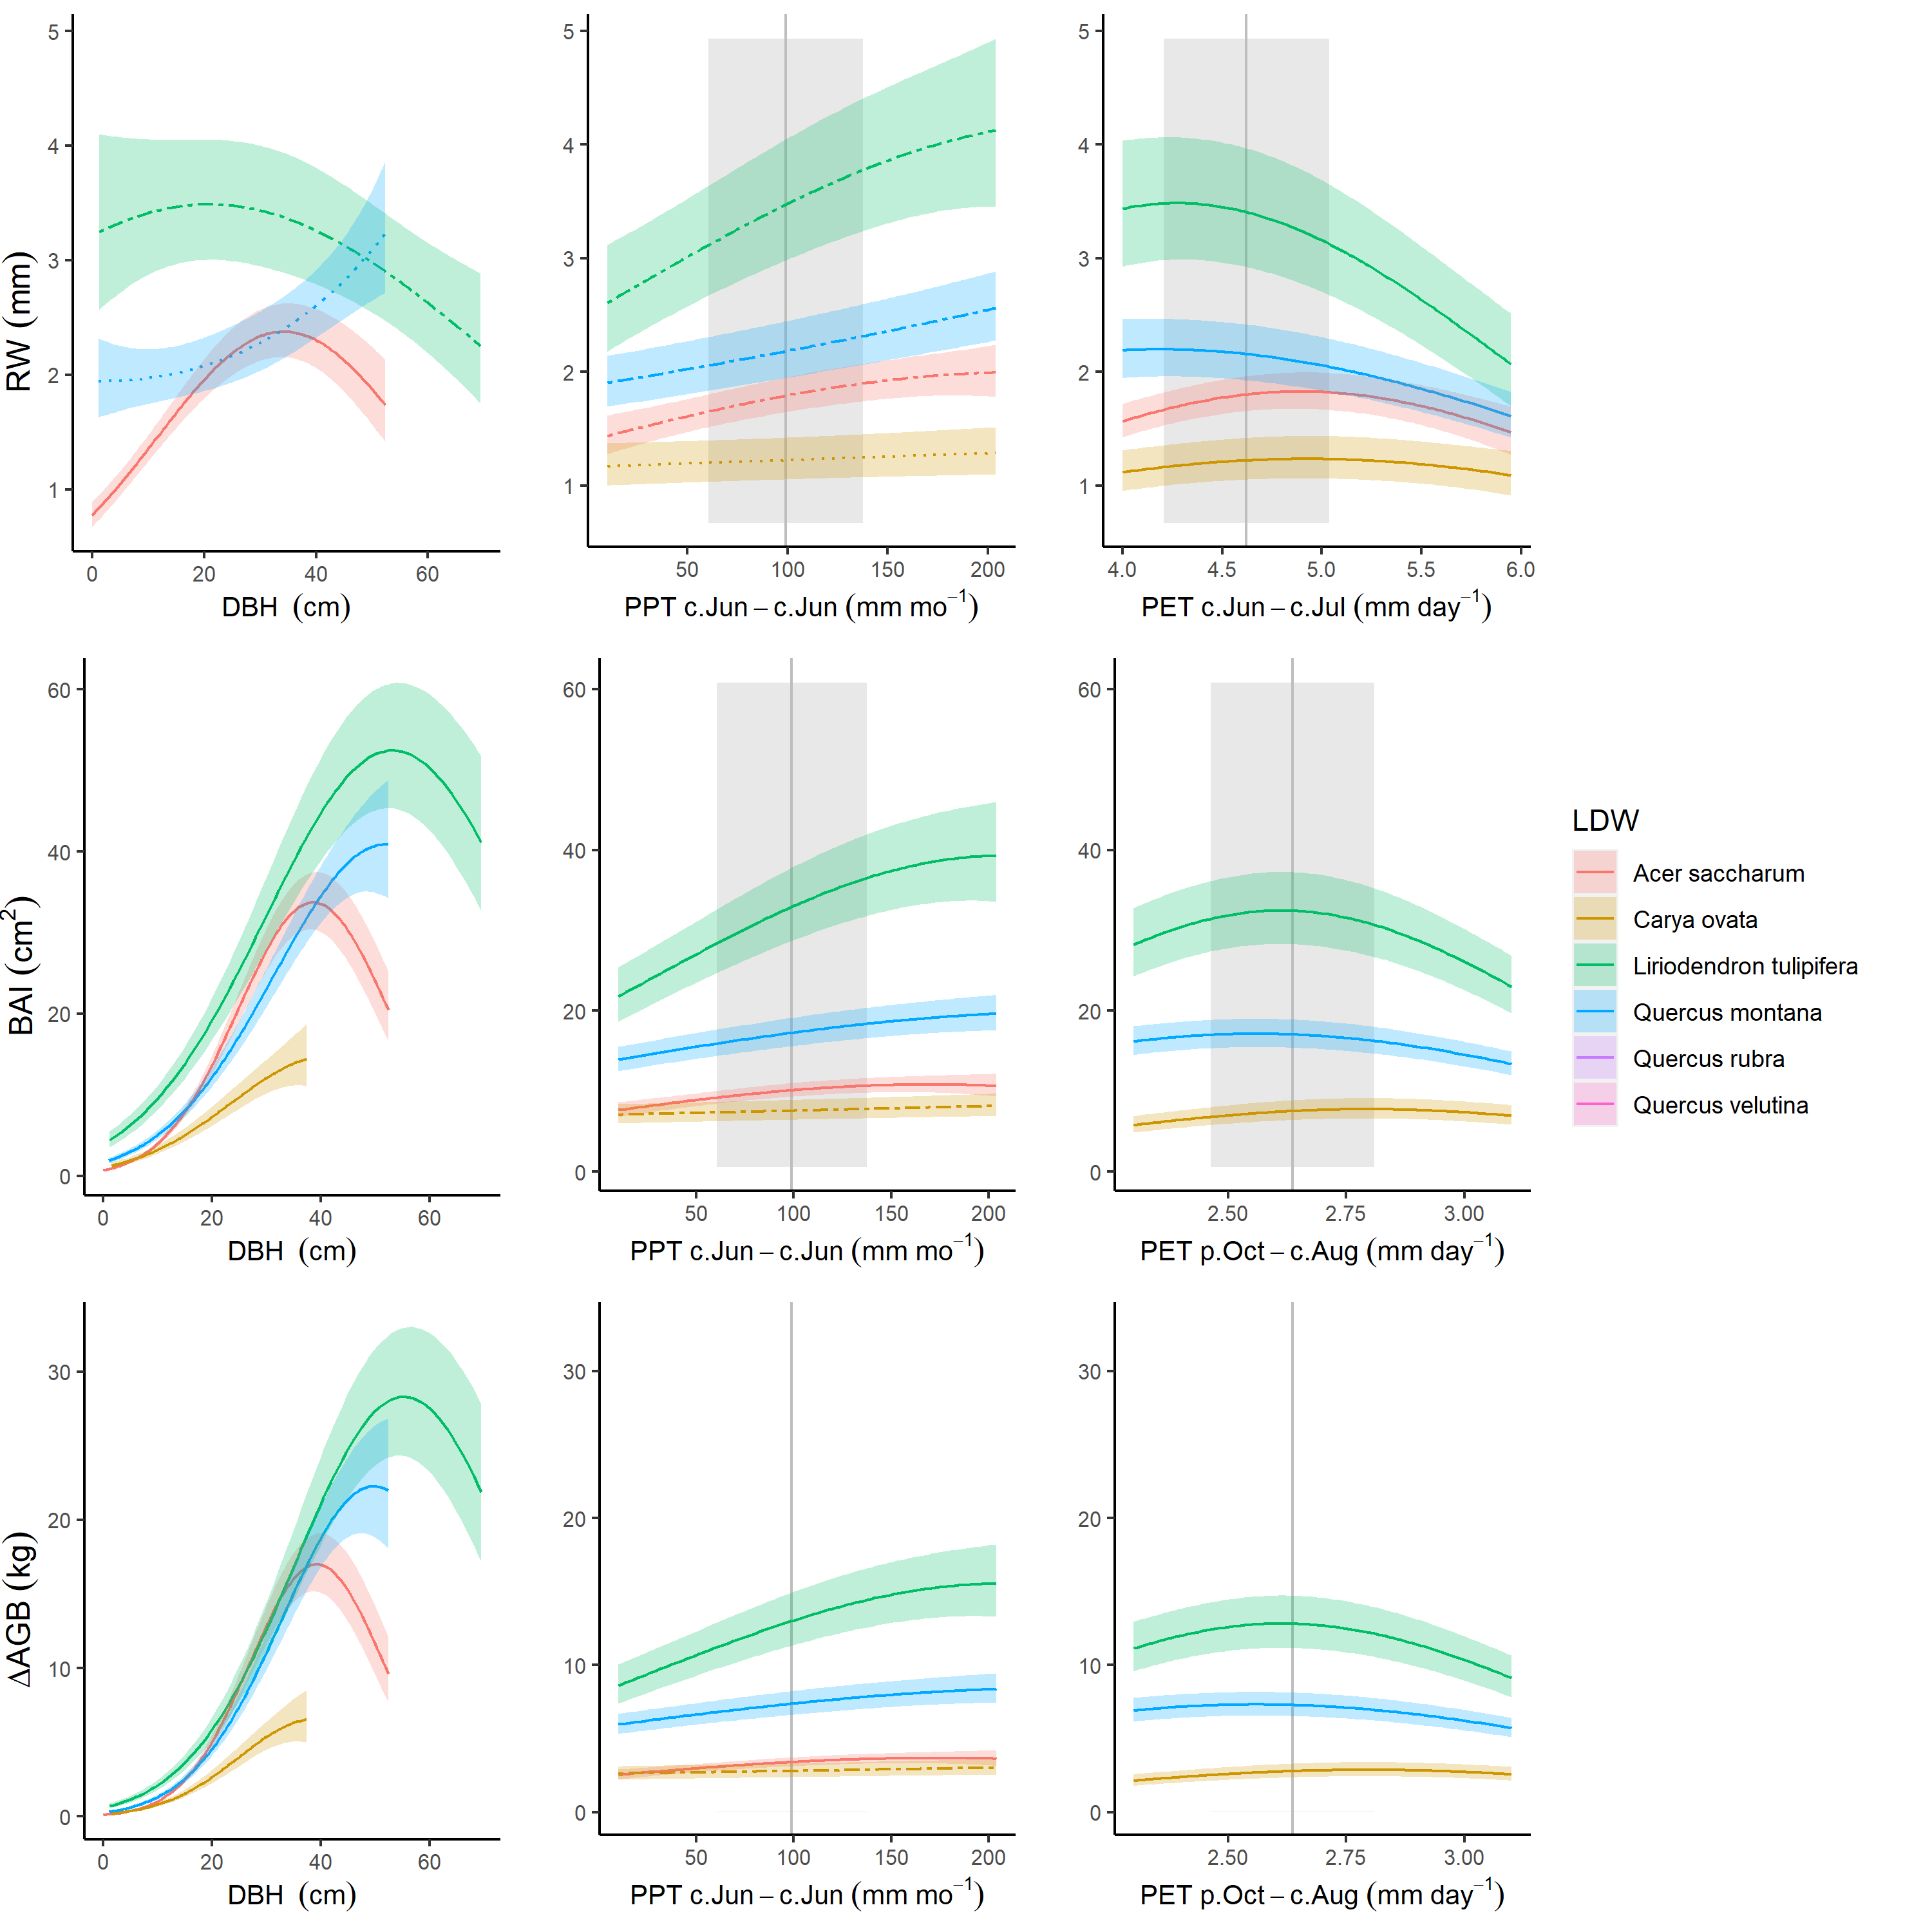
\includegraphics[width=0.78\textwidth,height=\textheight]{/Users/kteixeira/Dropbox (Smithsonian)/GitHub/EcoClimLab/ForestGEO-climate-sensitivity/results/composite_plots/LillyDickey.png}
\caption{\textbf{Figure S10 \textbar{} Best GLS models for Lilly Dickey
Woods (Indiana, USA) for all three growth metrics: \(\Delta r\),
\(BAI\), and \(\Delta AGB\).} Precipitation and temperature group
variables are as selected by \emph{climwin}. For each species,
relationships are plotted if included in top model, with dashed lines
indicating terms that do not significantly improve the model (relative
to a model without). Vertical grey lines indicate the long-term mean for
the climate variable, shading indicates 1 SD.}
\end{figure}

\newpage

\hypertarget{figure-s11.-best-gls-models-for-harvard-forest-massachusetts-usa}{%
\subsection{Figure S11. Best GLS models for Harvard Forest
(Massachusetts,
USA)}\label{figure-s11.-best-gls-models-for-harvard-forest-massachusetts-usa}}

\begin{figure}
\centering
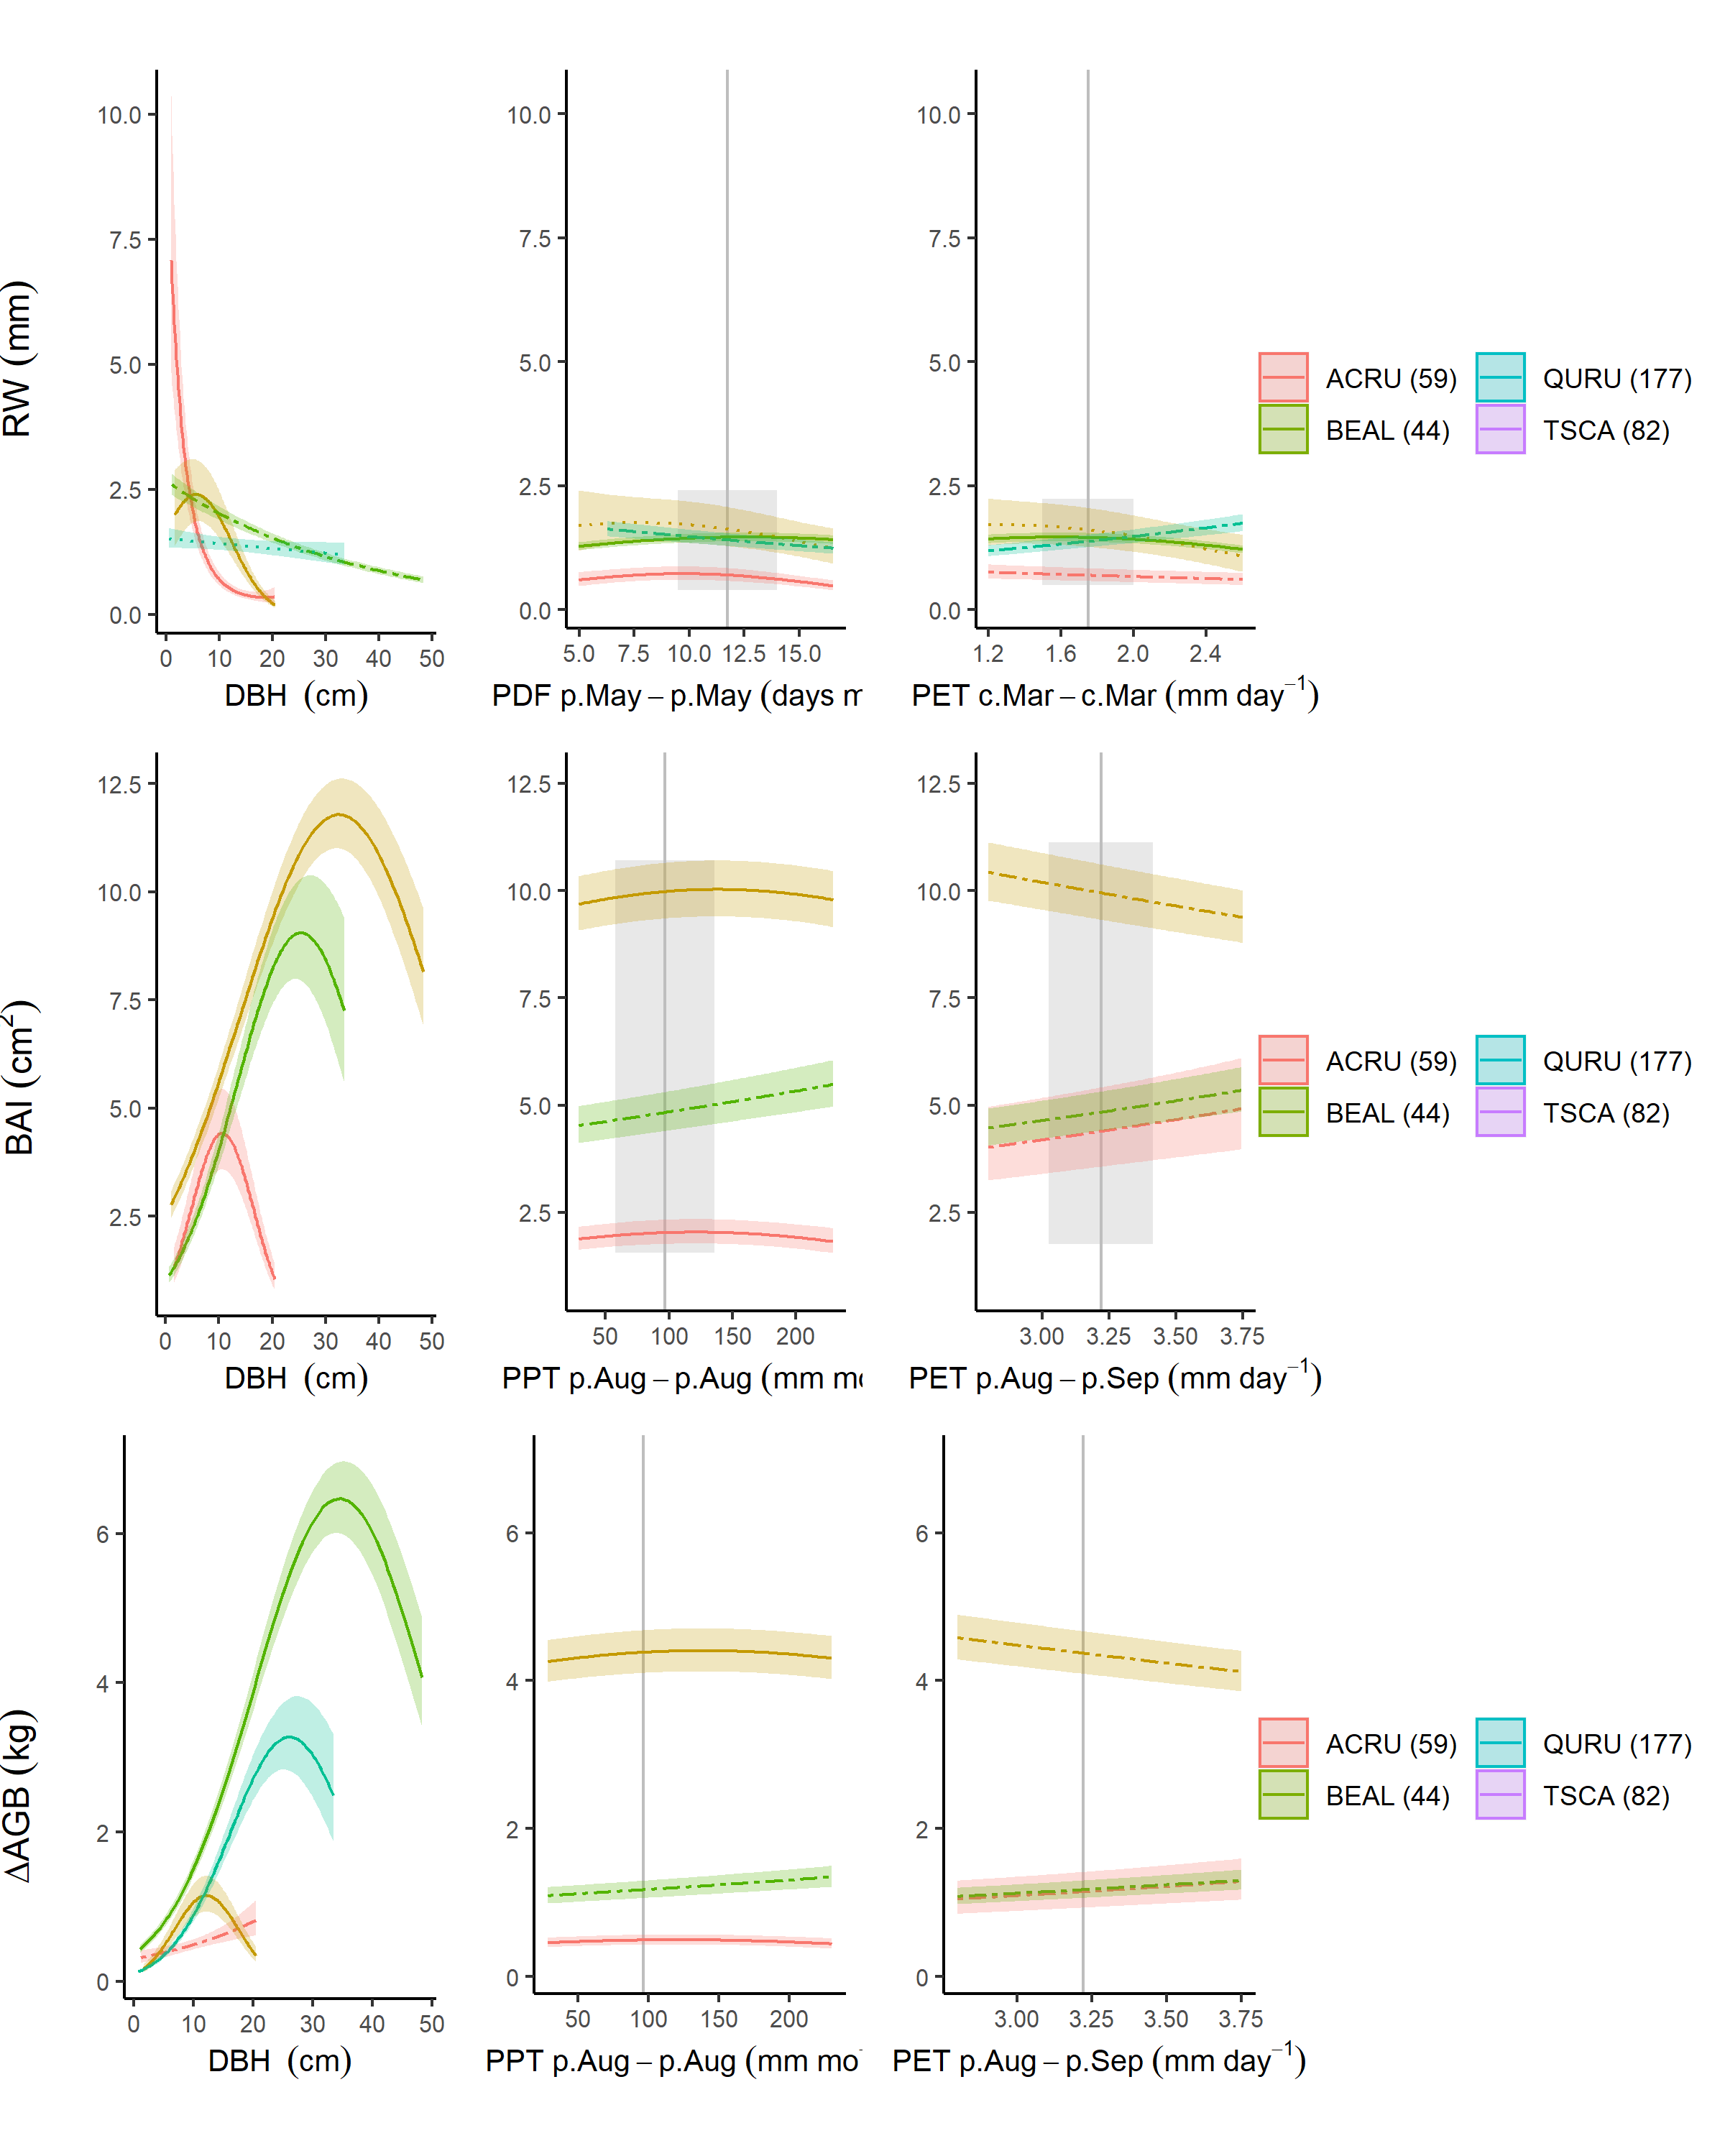
\includegraphics[width=0.78\textwidth,height=\textheight]{/Users/kteixeira/Dropbox (Smithsonian)/GitHub/EcoClimLab/ForestGEO-climate-sensitivity/results/composite_plots/HarvardForest.png}
\caption{\textbf{Figure S11 \textbar{} Best GLS models for Harvard
Forest (Massachusetts, USA) for all three growth metrics: \(\Delta r\),
\(BAI\), and \(\Delta AGB\).} Precipitation and temperature group
variables are as selected by \emph{climwin}. For each species,
relationships are plotted if included in top model, with dashed lines
indicating terms that do not significantly improve the model (relative
to a model without). Vertical grey lines indicate the long-term mean for
the climate variable, shading indicates 1 SD.}
\end{figure}

\newpage

\hypertarget{figure-s12.-best-gls-models-for-niobrara-hansley-nebraska-usa}{%
\subsection{Figure S12. Best GLS models for Niobrara/ Hansley (Nebraska,
USA)}\label{figure-s12.-best-gls-models-for-niobrara-hansley-nebraska-usa}}

\newpage

\hypertarget{figure-s13.-best-gls-models-for-zofin-czech-republic}{%
\subsection{Figure S13. Best GLS models for Zofin (Czech
Republic)}\label{figure-s13.-best-gls-models-for-zofin-czech-republic}}

\begin{figure}
\centering
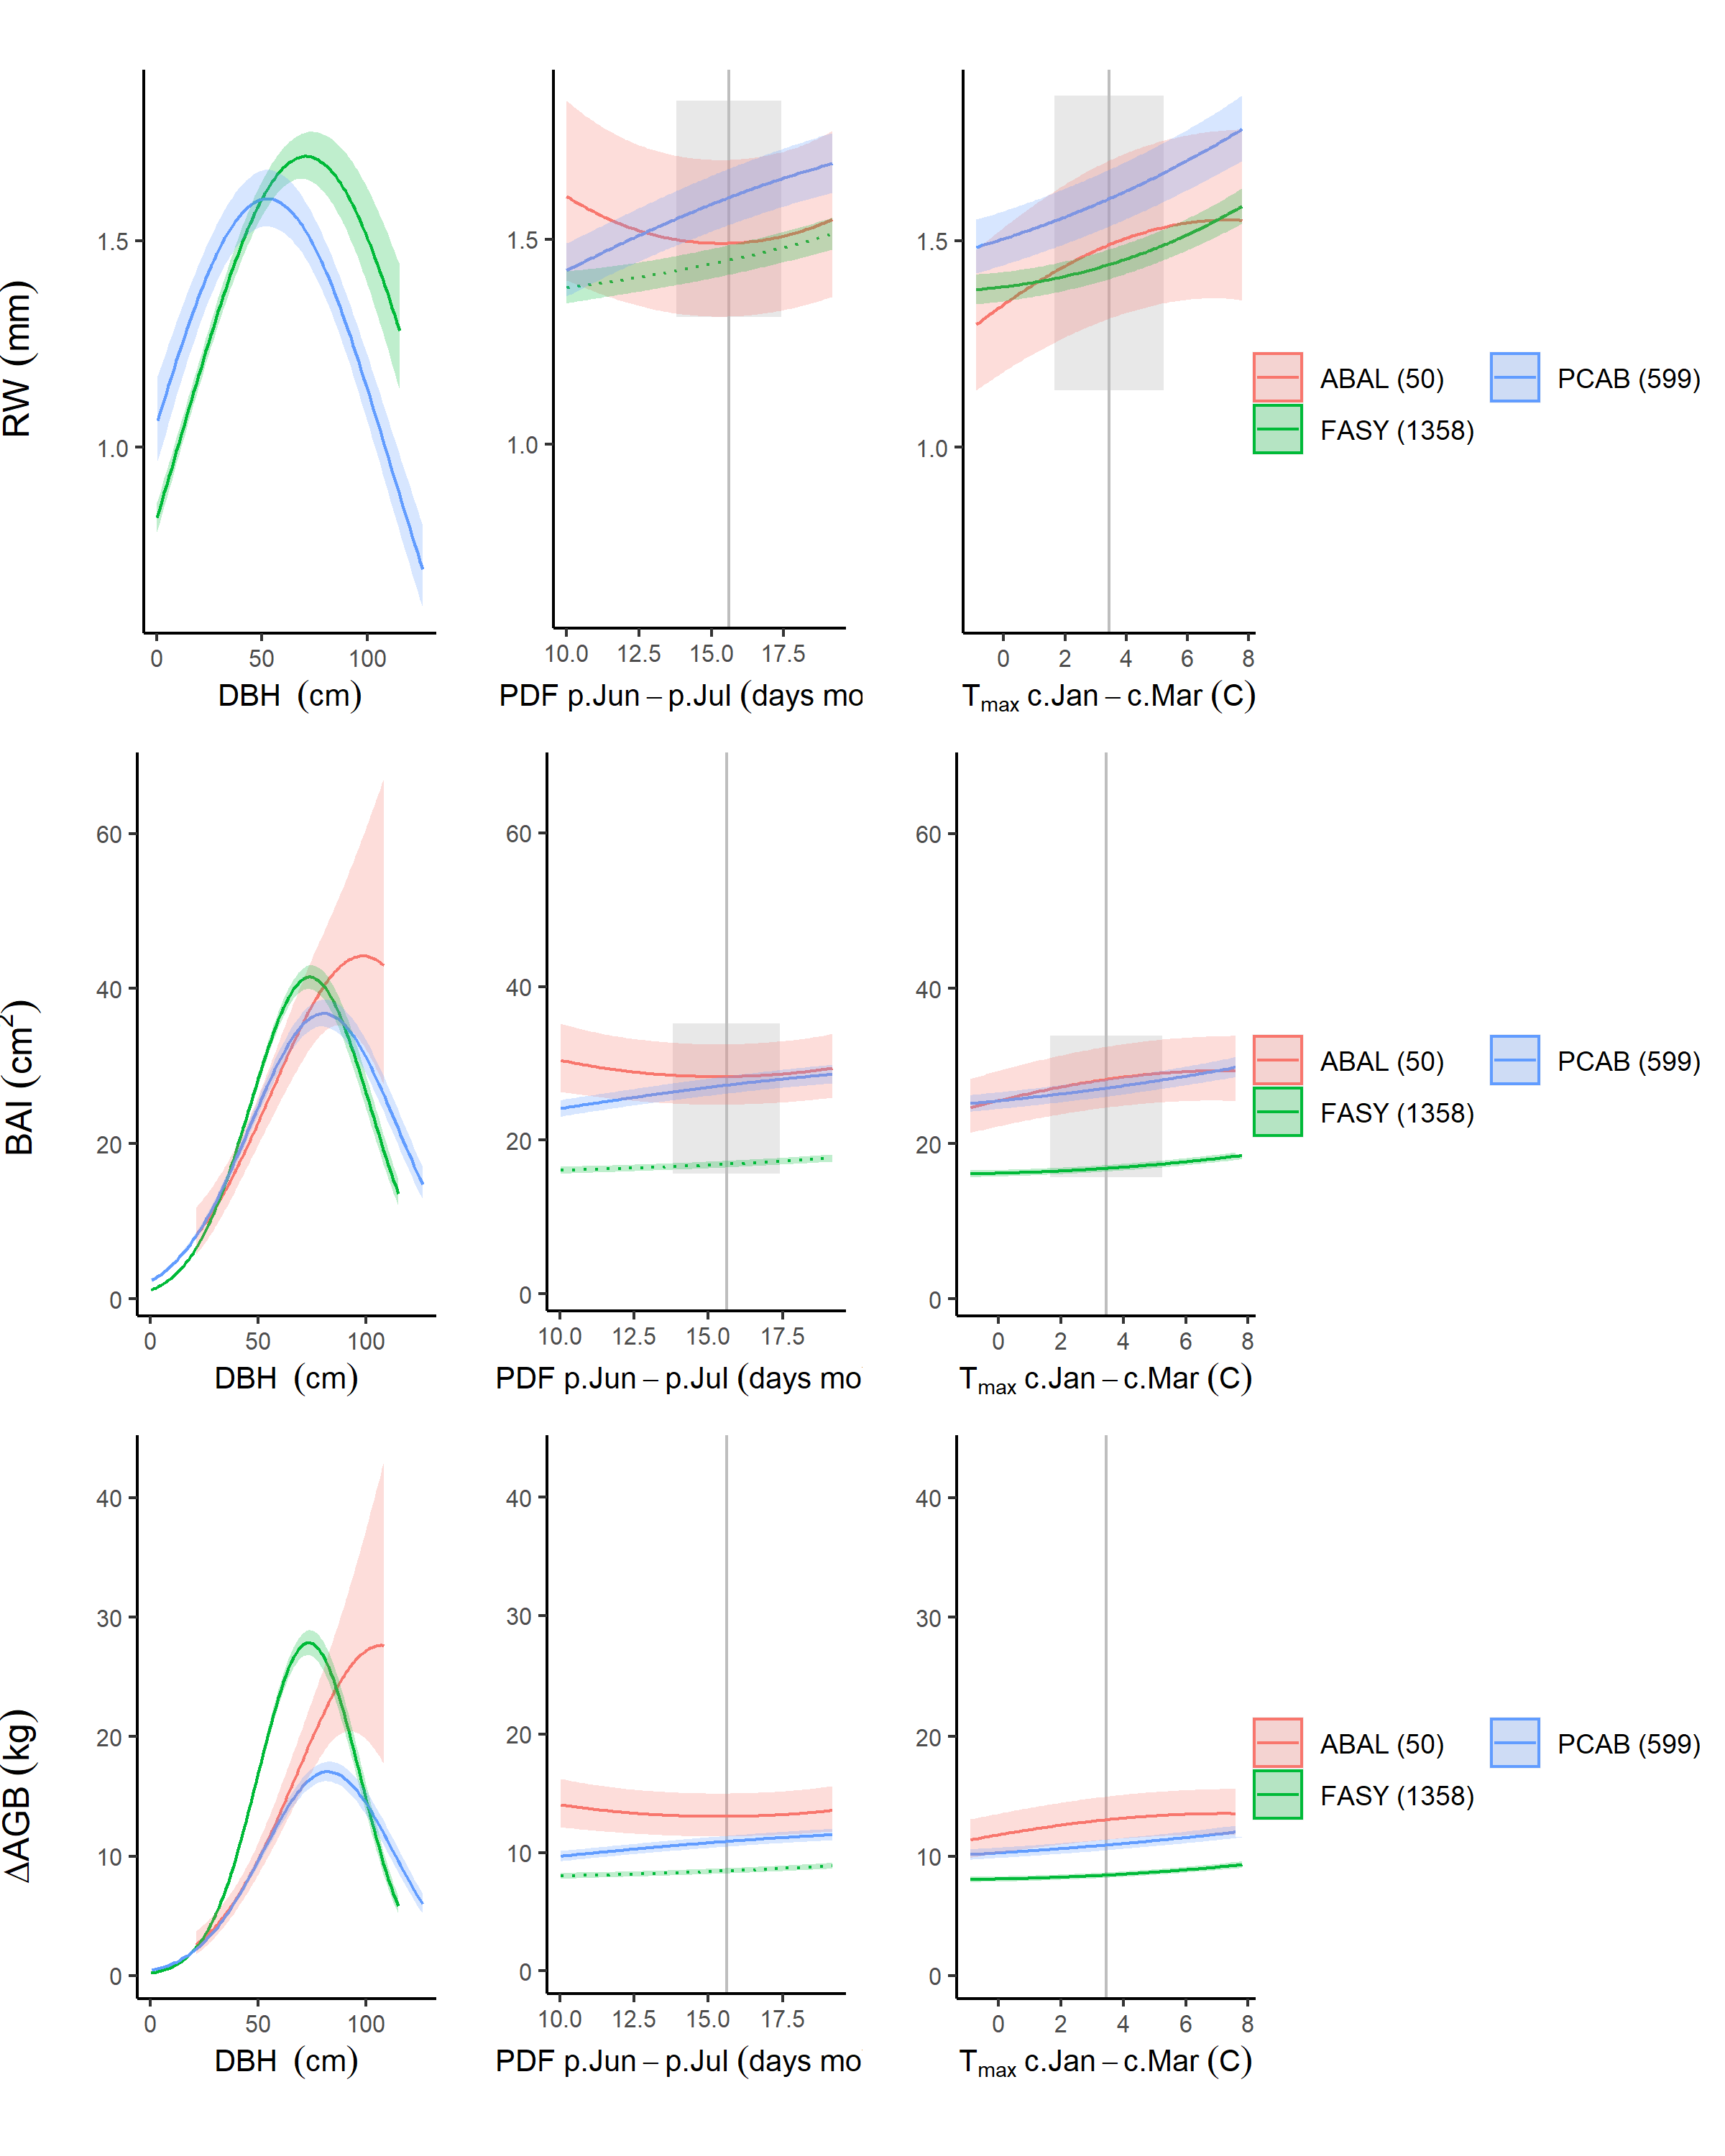
\includegraphics[width=0.78\textwidth,height=\textheight]{/Users/kteixeira/Dropbox (Smithsonian)/GitHub/EcoClimLab/ForestGEO-climate-sensitivity/results/composite_plots/Zofin.png}
\caption{\textbf{Figure S13 \textbar{} Best GLS models for Zofin (Czech
Republic) for all three growth metrics: \(\Delta r\), \(BAI\), and
\(\Delta AGB\).} Precipitation and temperature group variables are as
selected by \emph{climwin}. For each species, relationships are plotted
if included in top model, with dashed lines indicating terms that do not
significantly improve the model (relative to a model without). Vertical
grey lines indicate the long-term mean for the climate variable, shading
indicates 1 SD.}
\end{figure}

\newpage

\hypertarget{figure-s14.-best-gls-models-for-scotty-creek-nw-territories-canada}{%
\subsection{Figure S14. Best GLS models for Scotty Creek (NW
Territories,
Canada)}\label{figure-s14.-best-gls-models-for-scotty-creek-nw-territories-canada}}

\begin{figure}
\centering
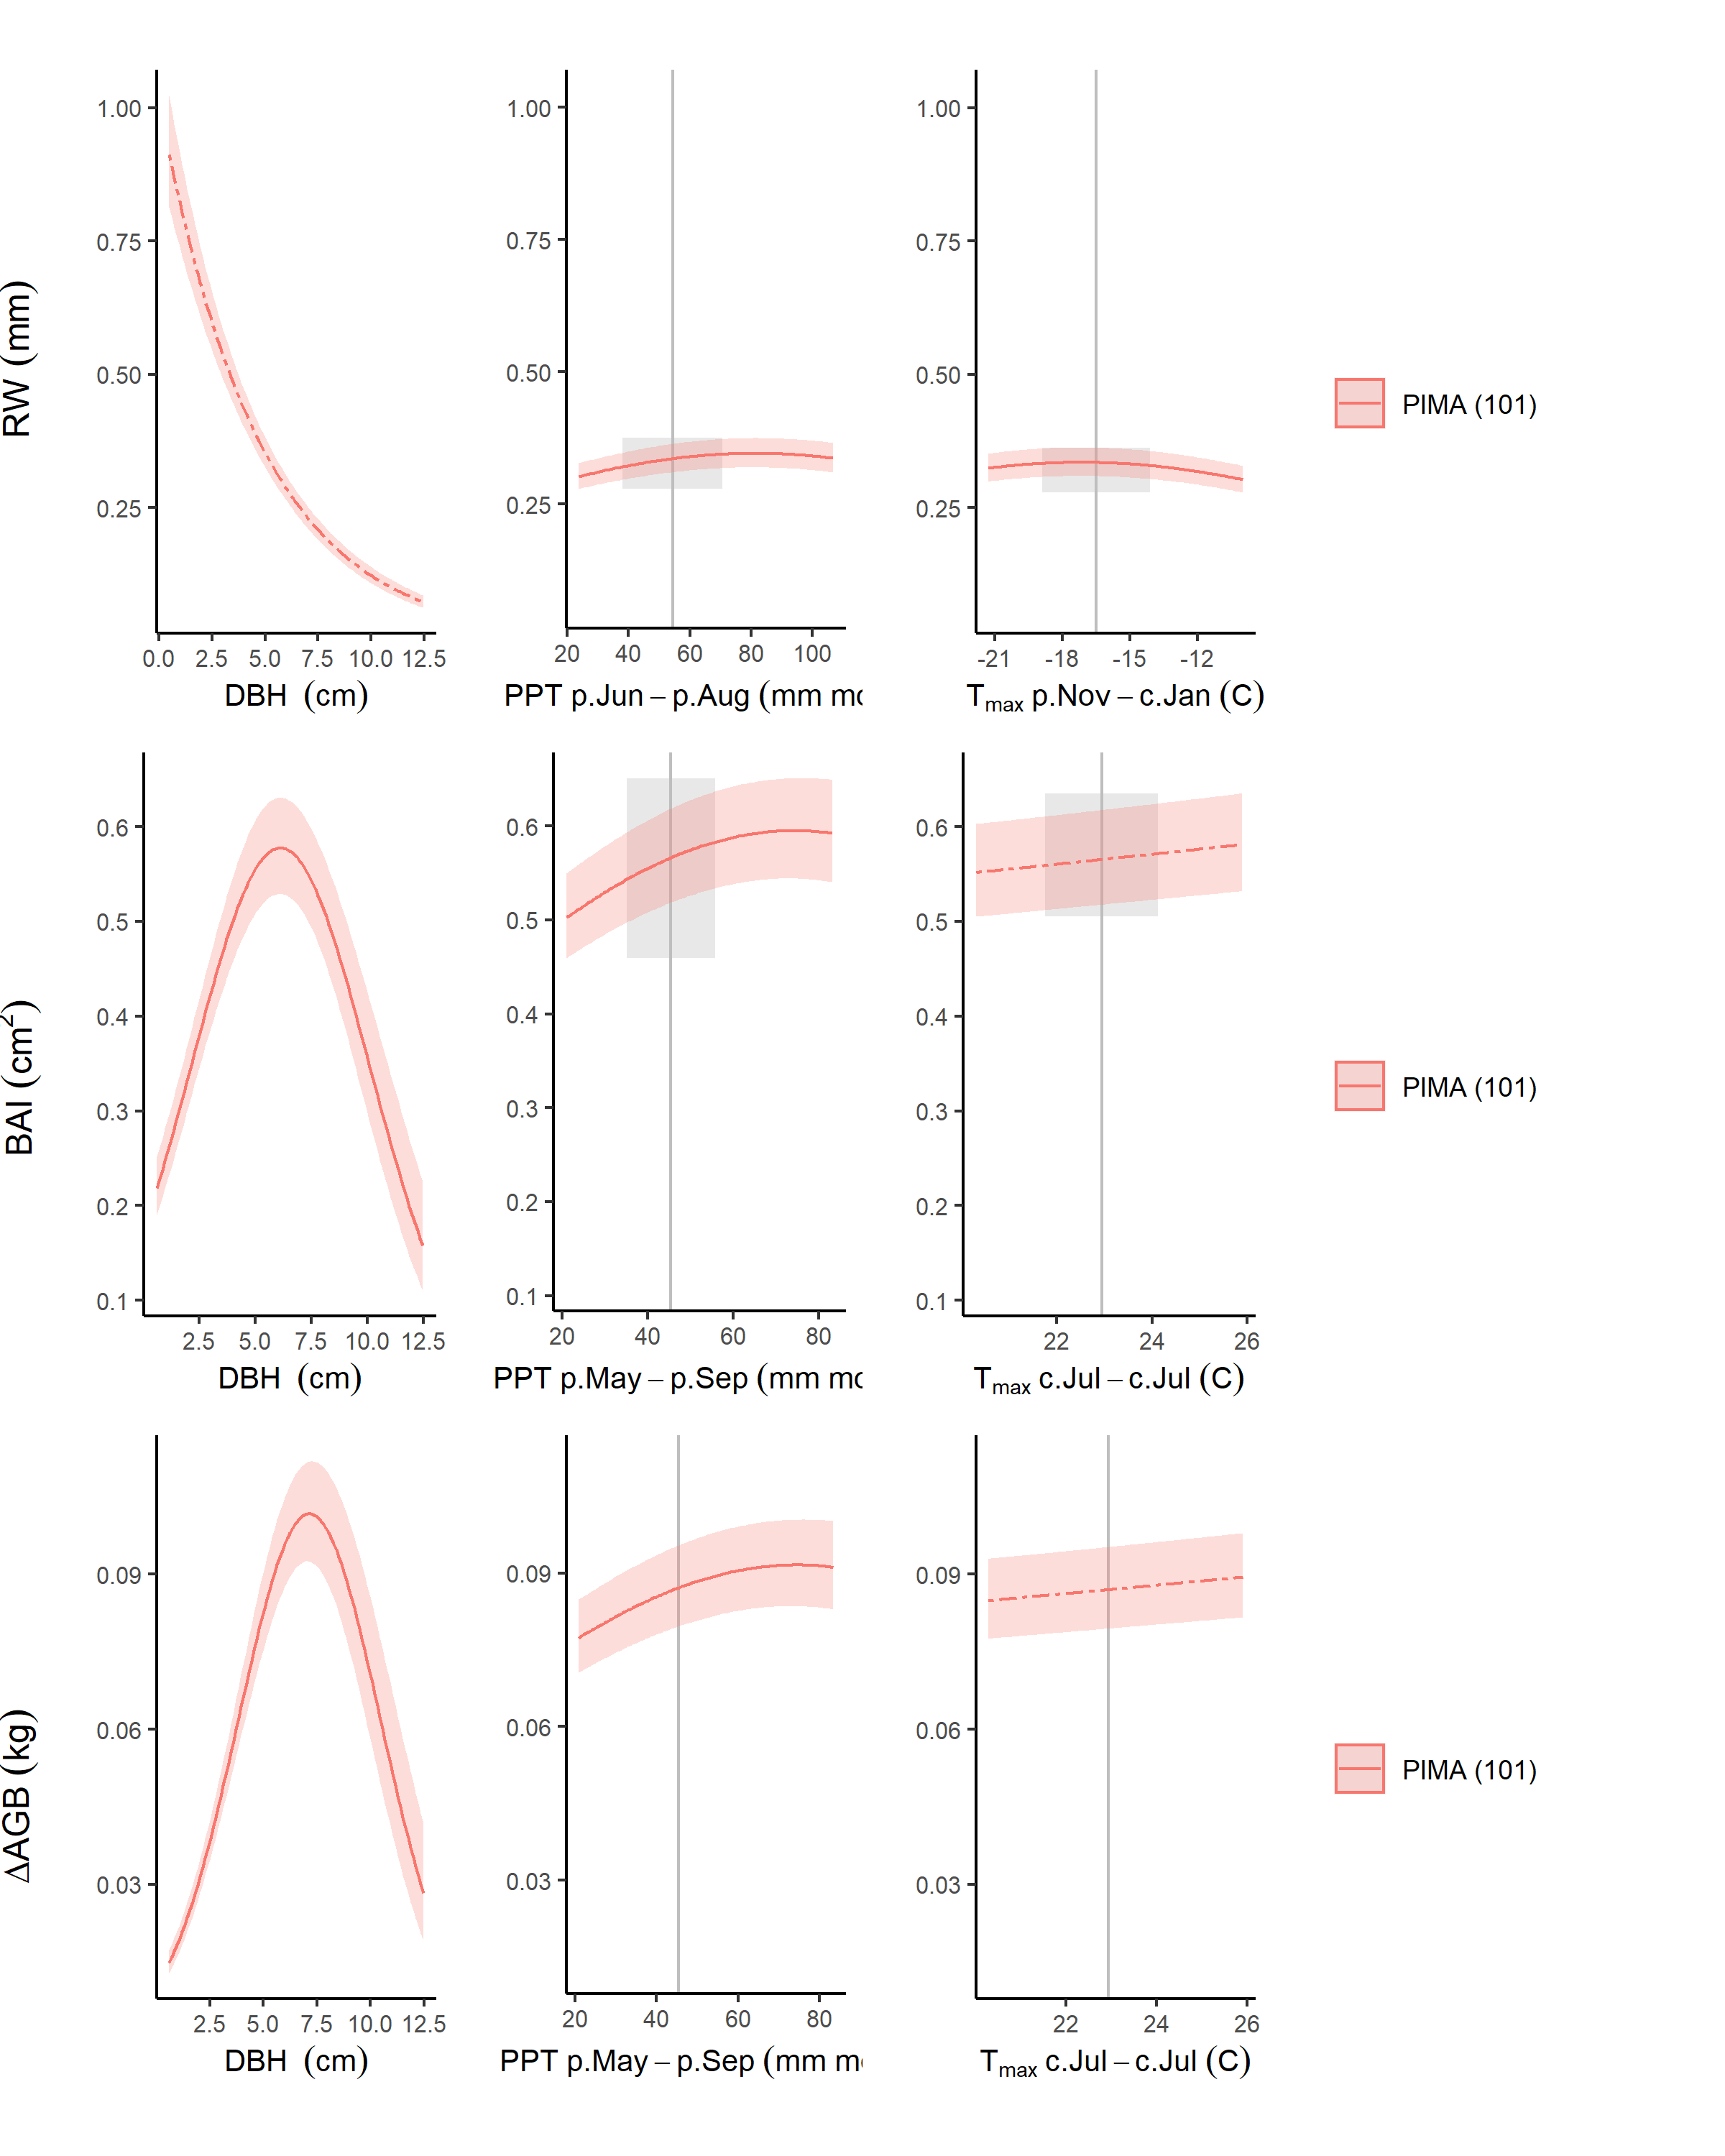
\includegraphics[width=0.78\textwidth,height=\textheight]{/Users/kteixeira/Dropbox (Smithsonian)/GitHub/EcoClimLab/ForestGEO-climate-sensitivity/results/composite_plots/ScottyCreek.png}
\caption{\textbf{Figure S14 \textbar{} Best GLS models for Scotty Creek
(NW Territories, Canada) for all three growth metrics: \(\Delta r\),
\(BAI\), and \(\Delta AGB\).} Precipitation and temperature group
variables are as selected by \emph{climwin}. For each species,
relationships are plotted if included in top model, with dashed lines
indicating terms that do not significantly improve the model (relative
to a model without). Vertical grey lines indicate the long-term mean for
the climate variable, shading indicates 1 SD.}
\end{figure}

\end{document}
